Das Ultraschall Phased Array wird bezüglich der Sende-Charakteristik, Empfangs-Charakteristik, Distanzauflösung und der maximalen Distanz getestet. Dabei wird jeweils der Messaufbau beschrieben und die Resultate dargestellt und kommentiert. Abschliessend sind ausgewählte Bilder von Umgebungsscans dargestellt und beschrieben. Die Anforderungen sind im Pflichtenheft (siehe \ref{sec:appendix_pflichtenheft}) im Abschnitt ''Ziele'' zu finden.

%%%%%%%%%%%%%%%%%%%%%%%%%%%%%%%%%%%%%%%%%%%%%%%%%%%%%%%%%%%%%%%%%%%%%%%%%%%%%%%%
%%%%%%%%%%%%%%%%%%%%%%%%%%%%%%%%%%%%%%%%%%%%%%%%%%%%%%%%%%%%%%%%%%%%%%%%%%%%%%%%
%%%%%%%%%%%%%%%%%%%%%%%%%%%%%%%%%%%%%%%%%%%%%%%%%%%%%%%%%%%%%%%%%%%%%%%%%%%%%%%%
\subsection{Messung der sendeseitigen Richtcharakteristik}\label{sec:messung_der_sendeseitigen_richtcharakteristik}
Die Richtcharakteristik des Sende-Arrays wird im reflexionsarmen Halbraum gemessen. Das Ultraschall Phased Array ist dabei auf einem Stativ befestigt und auf das Senden von acht Sendepulsen in einem bestimmten Winkel $\theta$ eingestellt. In einer Distanz von $2 \mathrm{m}$ befindet sich die Messschaltung. Sie liegt auf gleicher Höhe wie das Phased Array und ist auf dieses ausgerichtet. Die Messschaltung besteht dabei aus einem extern aufgebauten Kanal der Empfängerschaltung (siehe Kapitel \ref{sec:empfaengerschaltung}).
Das Ultraschall Phased Array-Gerät wird Grad für Grad im Bereich von $\alpha = \pm 45^{\circ}$ um die seine vertikale Achse gedreht. Die maximalen Spannungen der Wellenpakete, die an der Messschaltung auftreten, werden jeweils gemessen.

Der Messaufbau ist in Abbildung \ref{fig:image_test_messaufbau_0} zu sehen.

%%%%%%%%%%%%%%%%%%%%%%%%%%%%%%%%%%%%%%%%%%%%%%%%%%%%%%%%%%%%%%%%%%%%%%%%%%%%%%%%
% pictures
\begin{figure}[htb]
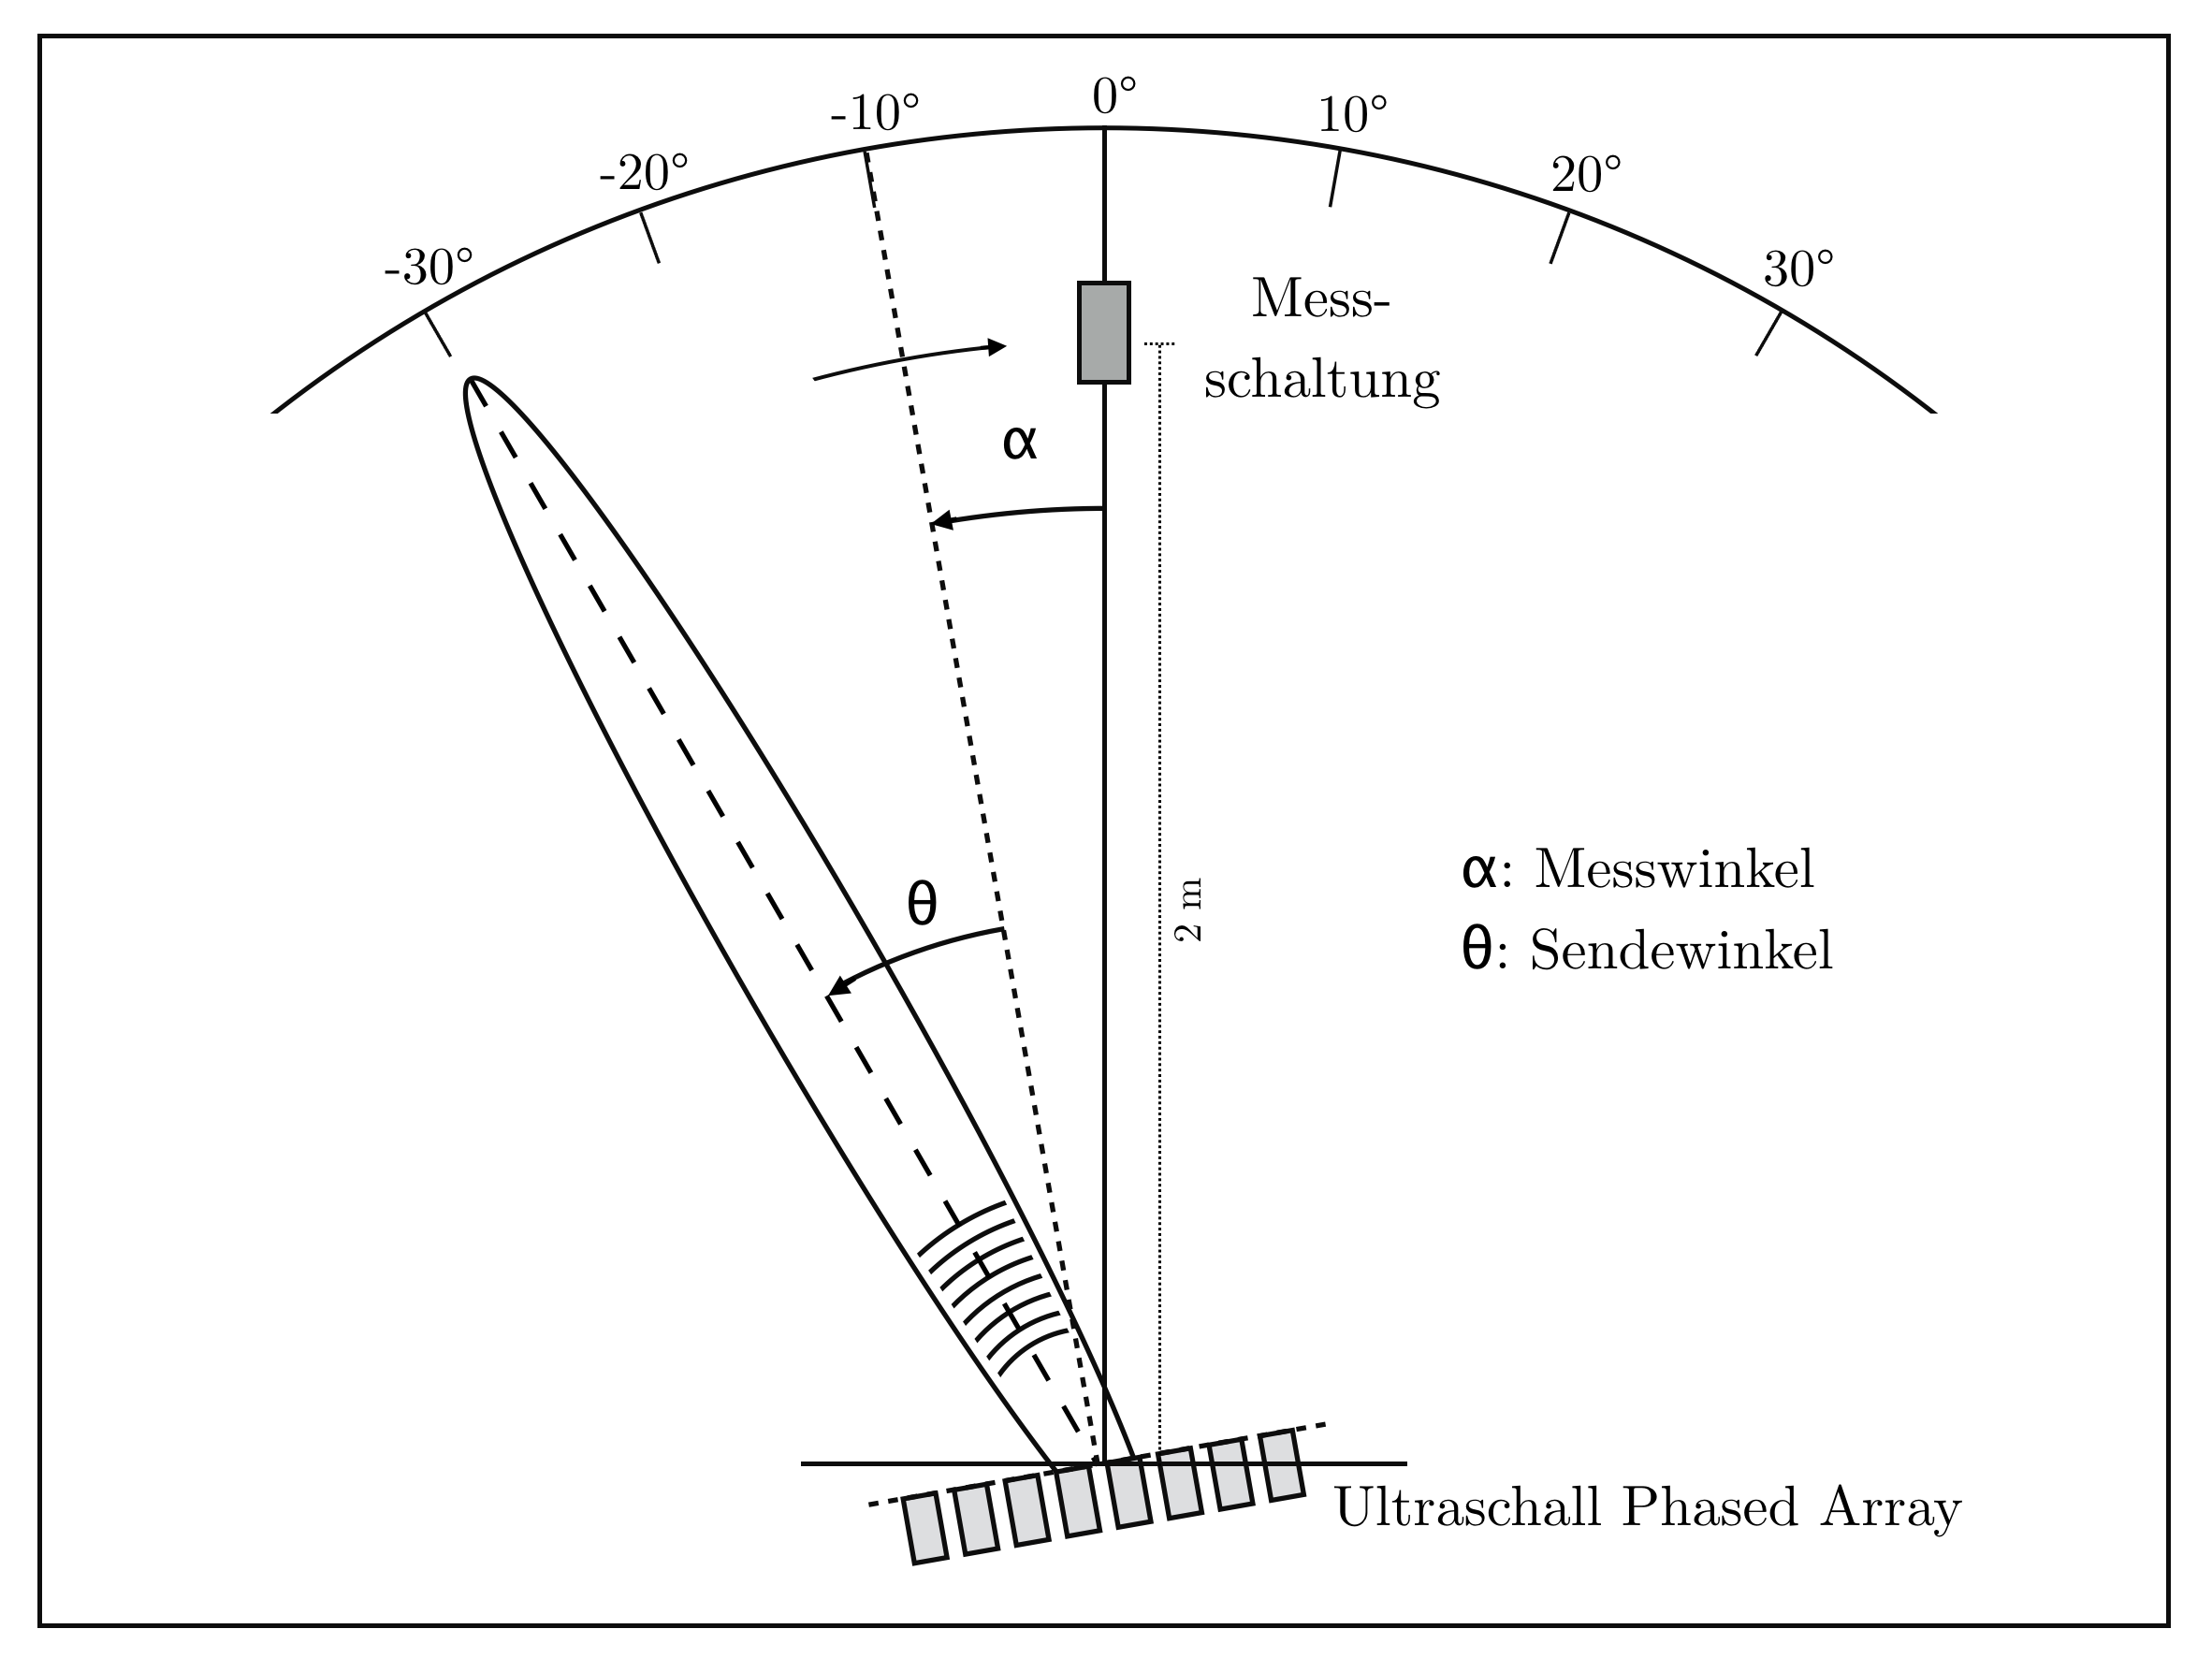
\includegraphics[width=\textwidth]{graphics/image_test_messaufbau_0.png}
\caption{Messaufbau im reflexionsarmen Halbraum} % picture caption
\label{fig:image_test_messaufbau_0}
\end{figure}
%
%(Abb. \ref{fig:image1})
%%%%%%%%%%%%%%%%%%%%%%%%%%%%%%%%%%%%%%%%%%%%%%%%%%%%%%%%%%%%%%%%%%%%%%%%%%%%%%%%

Die Messreihe für einen fest eingestellten Sendewinkel $\theta$ wird mit berechneten Werten verglichen (Formel \ref{eq:richtcharakteristik}).
Die Messwerte sind dabei auf den maximalen Wert der Messreihen normiert (bei $\theta = 0^{\circ}$ und $\alpha = 0^{\circ}$).

Die Ergebnisse sind in den Abbildungen \ref{fig:plot_test_characteristic_rect_0_polar}, \ref{fig:plot_test_characteristic_rect_10_polar}, \ref{fig:plot_test_characteristic_rect_20_polar} und \ref{fig:plot_test_characteristic_rect_30_polar} dargestellt.

\begin{figure}[htb]
\begin{minipage}{0.5\textwidth}
%%%%%%%%%%%%%%%%%%%%%%%%%%%%%%%%%%%%%%%%%%%%%%%%%%%%%%%%%%%%%%%%%%%%%%%%%%%%%%%%
% pictures
%\begin{figure}[htb]
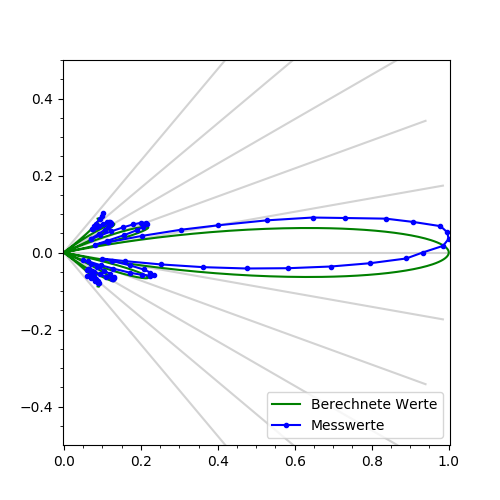
\includegraphics[width=\textwidth]{graphics/plot_test_characteristic_rect_0_polar.png}
\caption{Richtcharakteristik des Sende-Arrays bei einem Winkel von $\theta = 0^{\circ}$} % picture caption
\label{fig:plot_test_characteristic_rect_0_polar}
%\end{figure}
%
%(Abb. \ref{fig:image1})
%%%%%%%%%%%%%%%%%%%%%%%%%%%%%%%%%%%%%%%%%%%%%%%%%%%%%%%%%%%%%%%%%%%%%%%%%%%%%%%%
\end{minipage}
\begin{minipage}{0.5\textwidth}
%%%%%%%%%%%%%%%%%%%%%%%%%%%%%%%%%%%%%%%%%%%%%%%%%%%%%%%%%%%%%%%%%%%%%%%%%%%%%%%%
% pictures
%\begin{figure}[htb]
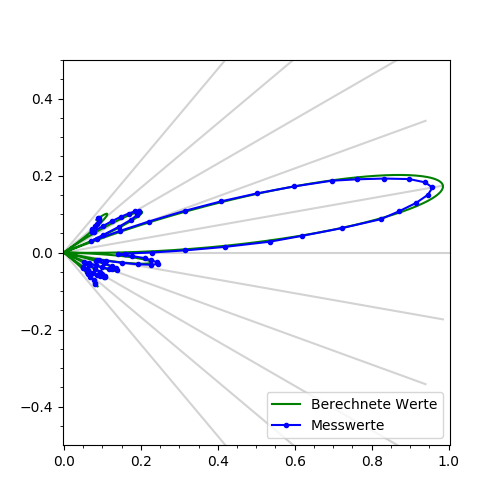
\includegraphics[width=\textwidth]{graphics/plot_test_characteristic_rect_10_polar.png}
\caption{Richtcharakteristik des Sende-Arrays bei einem Winkel von $\theta = 10^{\circ}$} % picture caption
\label{fig:plot_test_characteristic_rect_10_polar}
%\end{figure}
%
%(Abb. \ref{fig:image1})
%%%%%%%%%%%%%%%%%%%%%%%%%%%%%%%%%%%%%%%%%%%%%%%%%%%%%%%%%%%%%%%%%%%%%%%%%%%%%%%%
\end{minipage}
\begin{minipage}{0.5\textwidth}
%%%%%%%%%%%%%%%%%%%%%%%%%%%%%%%%%%%%%%%%%%%%%%%%%%%%%%%%%%%%%%%%%%%%%%%%%%%%%%%%
% pictures
%\begin{figure}[htb]
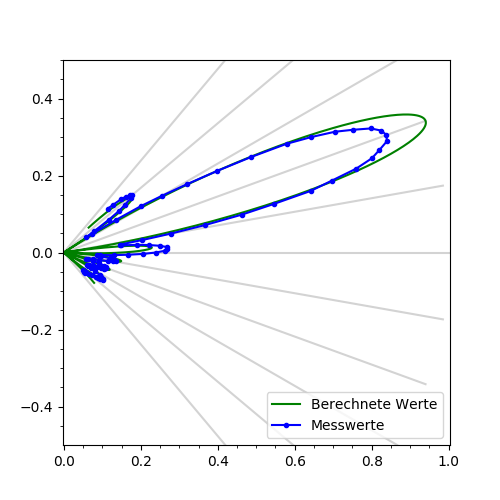
\includegraphics[width=\textwidth]{graphics/plot_test_characteristic_rect_20_polar.png}
\caption{Richtcharakteristik des Sende-Arrays bei einem Winkel von $\theta = 20^{\circ}$} % picture caption
\label{fig:plot_test_characteristic_rect_20_polar}
%\end{figure}
%
%(Abb. \ref{fig:image1})
%%%%%%%%%%%%%%%%%%%%%%%%%%%%%%%%%%%%%%%%%%%%%%%%%%%%%%%%%%%%%%%%%%%%%%%%%%%%%%%%
\end{minipage}
\begin{minipage}{0.5\textwidth}
%%%%%%%%%%%%%%%%%%%%%%%%%%%%%%%%%%%%%%%%%%%%%%%%%%%%%%%%%%%%%%%%%%%%%%%%%%%%%%%%
% pictures
%\begin{figure}[htb]
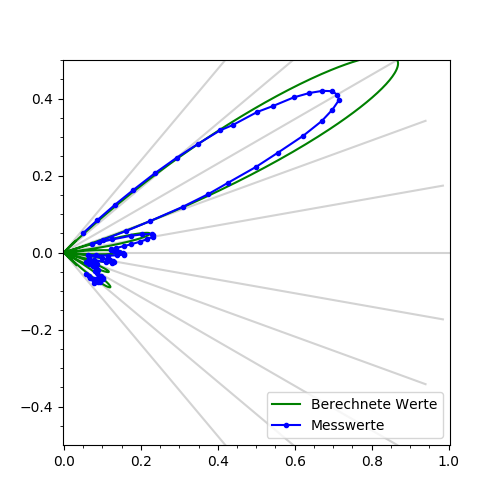
\includegraphics[width=\textwidth]{graphics/plot_test_characteristic_rect_30_polar.png}
\caption{Richtcharakteristik des Sende-Arrays bei einem Winkel von $\theta = 30^{\circ}$} % picture caption
\label{fig:plot_test_characteristic_rect_30_polar}
%\end{figure}
%
%(Abb. \ref{fig:image1})
%%%%%%%%%%%%%%%%%%%%%%%%%%%%%%%%%%%%%%%%%%%%%%%%%%%%%%%%%%%%%%%%%%%%%%%%%%%%%%%%
\end{minipage}
\end{figure}

Die Messresultate stimmen insgesamt gut mit den berechneten Werten überein. Die Abweichungen werden im Folgenden erklärt:

Da ein Rauschpegel vorhanden ist, sinken die Messungen nur auf einen gewissen minimalen Pegel.

In Abbildung \ref{fig:plot_test_characteristic_rect_0_polar} ist eine Abweichung von ca. $3^{\circ}$ zu sehen. Diese ist auf die minimale Verzögerungszeit zwischen dem Aktivieren der einzelnen PWM-Kanäle auf dem Mikrocontroller zurückzuführen. Diese Abweichung tritt im Bereich zwischen $\theta = \pm 2^{\circ}$ auf. In den Heatmap-Graphen im GUI äussert sich das Problem als Sprung um $0^{\circ}$, dies ist in Abbildung \ref{fig:image_test_obj_schaumstoff_0deg} zu sehen.

Da es sich bei den verwendeten Ultraschalltransceiver nicht um ideale Punktquellen handelt, nimmt der Schalldruck für grössere Sendewinkel ab. Dieses nicht-ideale Verhalten ist in Abbildung \ref{fig:plot_test_characteristic_rect_30_polar} gut zu sehen. Die Hauptkeule ist kleiner, die erste rechte Nebenkeule jedoch grösser als erwartet.

%\clearpage
%%%%%%%%%%%%%%%%%%%%%%%%%%%%%%%%%%%%%%%%%%%%%%%%%%%%%%%%%%%%%%%%%%%%%%%%%%%%%%%%
%%%%%%%%%%%%%%%%%%%%%%%%%%%%%%%%%%%%%%%%%%%%%%%%%%%%%%%%%%%%%%%%%%%%%%%%%%%%%%%%
%%%%%%%%%%%%%%%%%%%%%%%%%%%%%%%%%%%%%%%%%%%%%%%%%%%%%%%%%%%%%%%%%%%%%%%%%%%%%%%%
\subsection{Messung der sendeseitigen Richtcharakteristik mit Amplitudenbelegung}\label{sec:messung_der_sendeseitigen_richtcharakteristik_mit_amplitudenbelegung}
Mit dem gleichen Messaufbau aus Kapitel \ref{sec:messung_der_sendeseitigen_richtcharakteristik} wird die vom Mikrocontroller erzeugte Amplitudenbelegung (siehe letzter Abschnitt im Kapitel \ref{sec:ultraschall_sender}) gemessen. Dabei wird jeweils auf das Maximum der Messreihe normiert. Die theoretisch erreichbare Richtcharakteristik mit Amplitudenbelegung wurde mithilfe der Formel (\ref{eq:amplitudenbelegung}) aus dem Kapitel \ref{sec:amplitudenbelegung} berechnet.

\begin{figure}[htb]
\begin{minipage}{0.5\textwidth}
%%%%%%%%%%%%%%%%%%%%%%%%%%%%%%%%%%%%%%%%%%%%%%%%%%%%%%%%%%%%%%%%%%%%%%%%%%%%%%%%
% pictures
%\begin{figure}[htb]
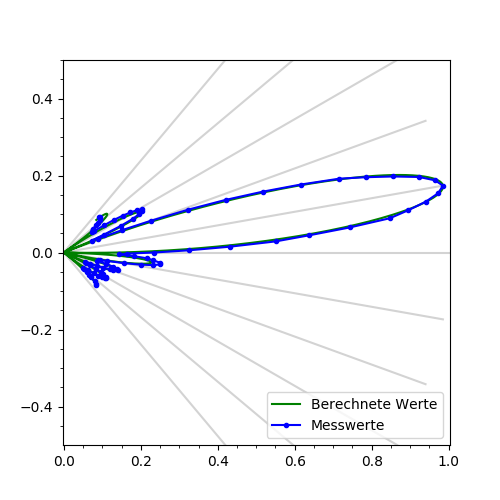
\includegraphics[width=\textwidth]{graphics/plot_test_characteristic_aperture_0_polar.png}
\caption{Richtcharakteristik des Sende-Arrays für eine Rechteckbelegung und $\theta = 10$ Grad} % picture caption
\label{fig:plot_test_characteristic_aperture_0_polar}
%\end{figure}
%
%(Abb. \ref{fig:image1})
%%%%%%%%%%%%%%%%%%%%%%%%%%%%%%%%%%%%%%%%%%%%%%%%%%%%%%%%%%%%%%%%%%%%%%%%%%%%%%%%
\end{minipage}
\begin{minipage}{0.5\textwidth}
%%%%%%%%%%%%%%%%%%%%%%%%%%%%%%%%%%%%%%%%%%%%%%%%%%%%%%%%%%%%%%%%%%%%%%%%%%%%%%%%
% pictures
%\begin{figure}[htb]
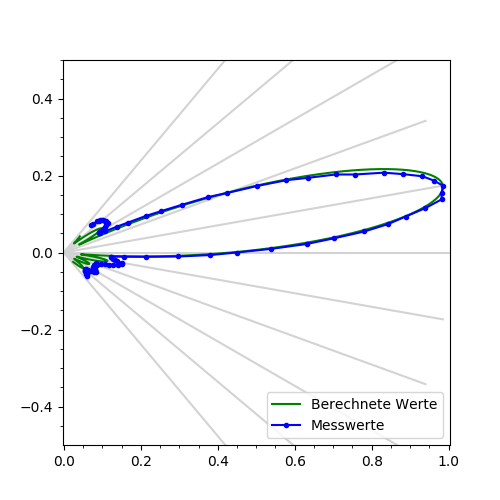
\includegraphics[width=\textwidth]{graphics/plot_test_characteristic_aperture_1_polar.png}
\caption{Richtcharakteristik des Sende-Arrays für eine $\cos$-Belegung und $\theta = 10$ Grad} % picture caption
\label{fig:plot_test_characteristic_aperture_1_polar}
%\end{figure}
%
%(Abb. \ref{fig:image1})
%%%%%%%%%%%%%%%%%%%%%%%%%%%%%%%%%%%%%%%%%%%%%%%%%%%%%%%%%%%%%%%%%%%%%%%%%%%%%%%%
\end{minipage}
\begin{minipage}{0.5\textwidth}
%%%%%%%%%%%%%%%%%%%%%%%%%%%%%%%%%%%%%%%%%%%%%%%%%%%%%%%%%%%%%%%%%%%%%%%%%%%%%%%%
% pictures
%\begin{figure}[htb]
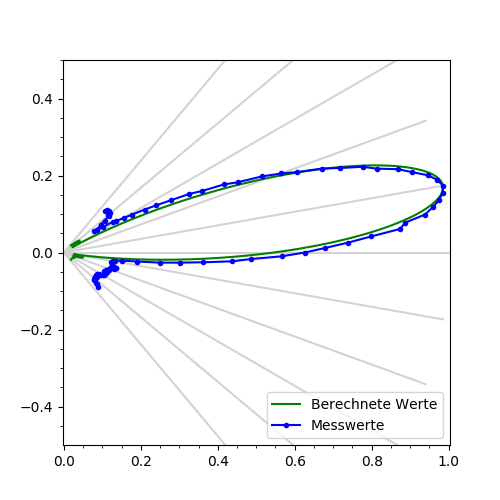
\includegraphics[width=\textwidth]{graphics/plot_test_characteristic_aperture_2_polar.png}
\caption{Richtcharakteristik des Sende-Arrays für eine $\cos^2$-Belegung und $\theta = 10$ Grad} % picture caption
\label{fig:plot_test_characteristic_aperture_2_polar}
%\end{figure}
%
%(Abb. \ref{fig:image1})
%%%%%%%%%%%%%%%%%%%%%%%%%%%%%%%%%%%%%%%%%%%%%%%%%%%%%%%%%%%%%%%%%%%%%%%%%%%%%%%%
\end{minipage}
\begin{minipage}{0.5\textwidth}
%%%%%%%%%%%%%%%%%%%%%%%%%%%%%%%%%%%%%%%%%%%%%%%%%%%%%%%%%%%%%%%%%%%%%%%%%%%%%%%%
% pictures
%\begin{figure}[htb]
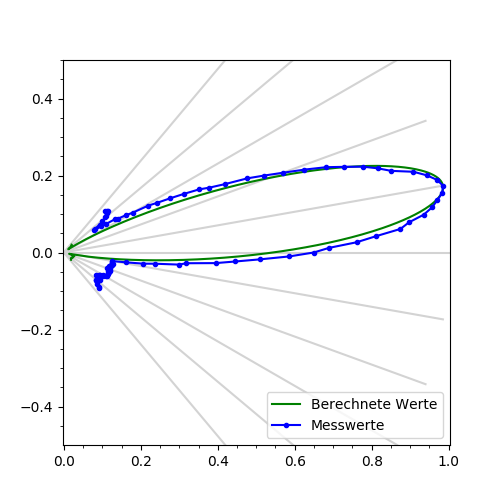
\includegraphics[width=\textwidth]{graphics/plot_test_characteristic_aperture_3_polar.png}
\caption{Richtcharakteristik des Sende-Arrays für eine Gaussbelegung und $\theta = 10$ Grad} % picture caption
\label{fig:plot_test_characteristic_aperture_3_polar}
%\end{figure}
%
%(Abb. \ref{fig:image1})
%%%%%%%%%%%%%%%%%%%%%%%%%%%%%%%%%%%%%%%%%%%%%%%%%%%%%%%%%%%%%%%%%%%%%%%%%%%%%%%%
\end{minipage}
\end{figure}

Die gemessenen Hauptkeulen mit Amplitudenbelegung in den Abbildungen \ref{fig:plot_test_characteristic_aperture_1_polar}, \ref{fig:plot_test_characteristic_aperture_2_polar} und \ref{fig:plot_test_characteristic_aperture_3_polar} sind breiter als die Hauptkeule in Abbildung \ref{fig:plot_test_characteristic_aperture_0_polar} mit Rechteckbelegung, was der Theorie entspricht. Da die Messungen auf das Maximum normiert sind, die Sendeleistung jedoch insgesamt verkleinert wird, hebt sich der Rauschpegel. Die Nebenkeulen sind zwar gedämpft, jedoch nicht so stark wie berechnet. Dies könnte auf mechanische Kopplung zwischen den Sendern und/oder kleinere mechanische Ungenauigkeiten beim Auflöten der Ultraschalltransceiver zurückzuführen sein.

\clearpage
%%%%%%%%%%%%%%%%%%%%%%%%%%%%%%%%%%%%%%%%%%%%%%%%%%%%%%%%%%%%%%%%%%%%%%%%%%%%%%%%
%%%%%%%%%%%%%%%%%%%%%%%%%%%%%%%%%%%%%%%%%%%%%%%%%%%%%%%%%%%%%%%%%%%%%%%%%%%%%%%%
%%%%%%%%%%%%%%%%%%%%%%%%%%%%%%%%%%%%%%%%%%%%%%%%%%%%%%%%%%%%%%%%%%%%%%%%%%%%%%%%
\subsection{Messung der empfangsseitigen Richtcharakteristik}\label{sec:messung_der_empfangsseitigen_richtcharakteristik}

Werden die acht empfangenen Signale vor der Addition zeitlich korrekt verschoben, entsteht auch empfängerseitig eine Richtcharakteristik (siehe Kapitel \ref{sec:beamforming}). Für den Messaufbau wird das Ultraschall Phased Array auf einem Stativ in $2 \mathrm{m}$ Distanz vor einer gut reflektierenden Oberfläche (Wand) aufgestellt.  Bodenreflexionen werden mit einem Schaumstoffstück verhindert.

Es wird daraufhin das Gerät auf einem Stativ so ausgerichtet, dass der Schall eines Sendevorgangs mit dem Sendewinkel $\theta$ senkrecht auf der Wand auftrifft. Danach trifft der reflektierte Schall wieder mit dem gleichen Winkel auf das Array auf. Der Messaufbau ist in Abbildung \ref{fig:image_test_messaufbau_1} zu sehen.
Nach einem Sendevorgang in diesem Winkel $\theta$ werden die acht empfangenen Signale gespeichert. Um Störungen zu vermeiden werden die ersten Werte dieser Signale abgeschnitten. Danach werden die Signale für jeden empfangsseitigen Winkel zwischen $\pm 90^{\circ}$ aufaddiert. Dies geschieht mithilfe der Funktion \texttt{upsamp\_beam\_form(\dots)} (siehe Kapitel \ref{sec:signalverarbeitung}).
Aus den daraus resultierenden Wellenpaketen wird jeweils das Maximum ausgelesen.
Werden diese Maxima zum zugehörigen Winkel aufgetragen, entsteht so die empfangsseitige Richtcharakteristik. Diese Messung wird nach korrekter Positionierung des Phased Arrays über das Pythonskript ''testing.py'' durchgeführt, dabei werden die Graphen automatisch erzeugt. Mit \texttt{python ./software/server\_flask/testing.py -{}-help} kann eine Bedienungsanleitung dieser Funktion aufgerufen werden. Die Messwerte sind jeweils dabei auf den maximalen Wert der Messreihe normiert.

Die empfangsseitige Amplitudenbelegung (siehe Kapitel \ref{sec:amplitudenbelegung}) wird durch entsprechendes Gewichten der Signale vor der Addition erzielt.

%%%%%%%%%%%%%%%%%%%%%%%%%%%%%%%%%%%%%%%%%%%%%%%%%%%%%%%%%%%%%%%%%%%%%%%%%%%%%%%%
% pictures
\begin{figure}[htb]
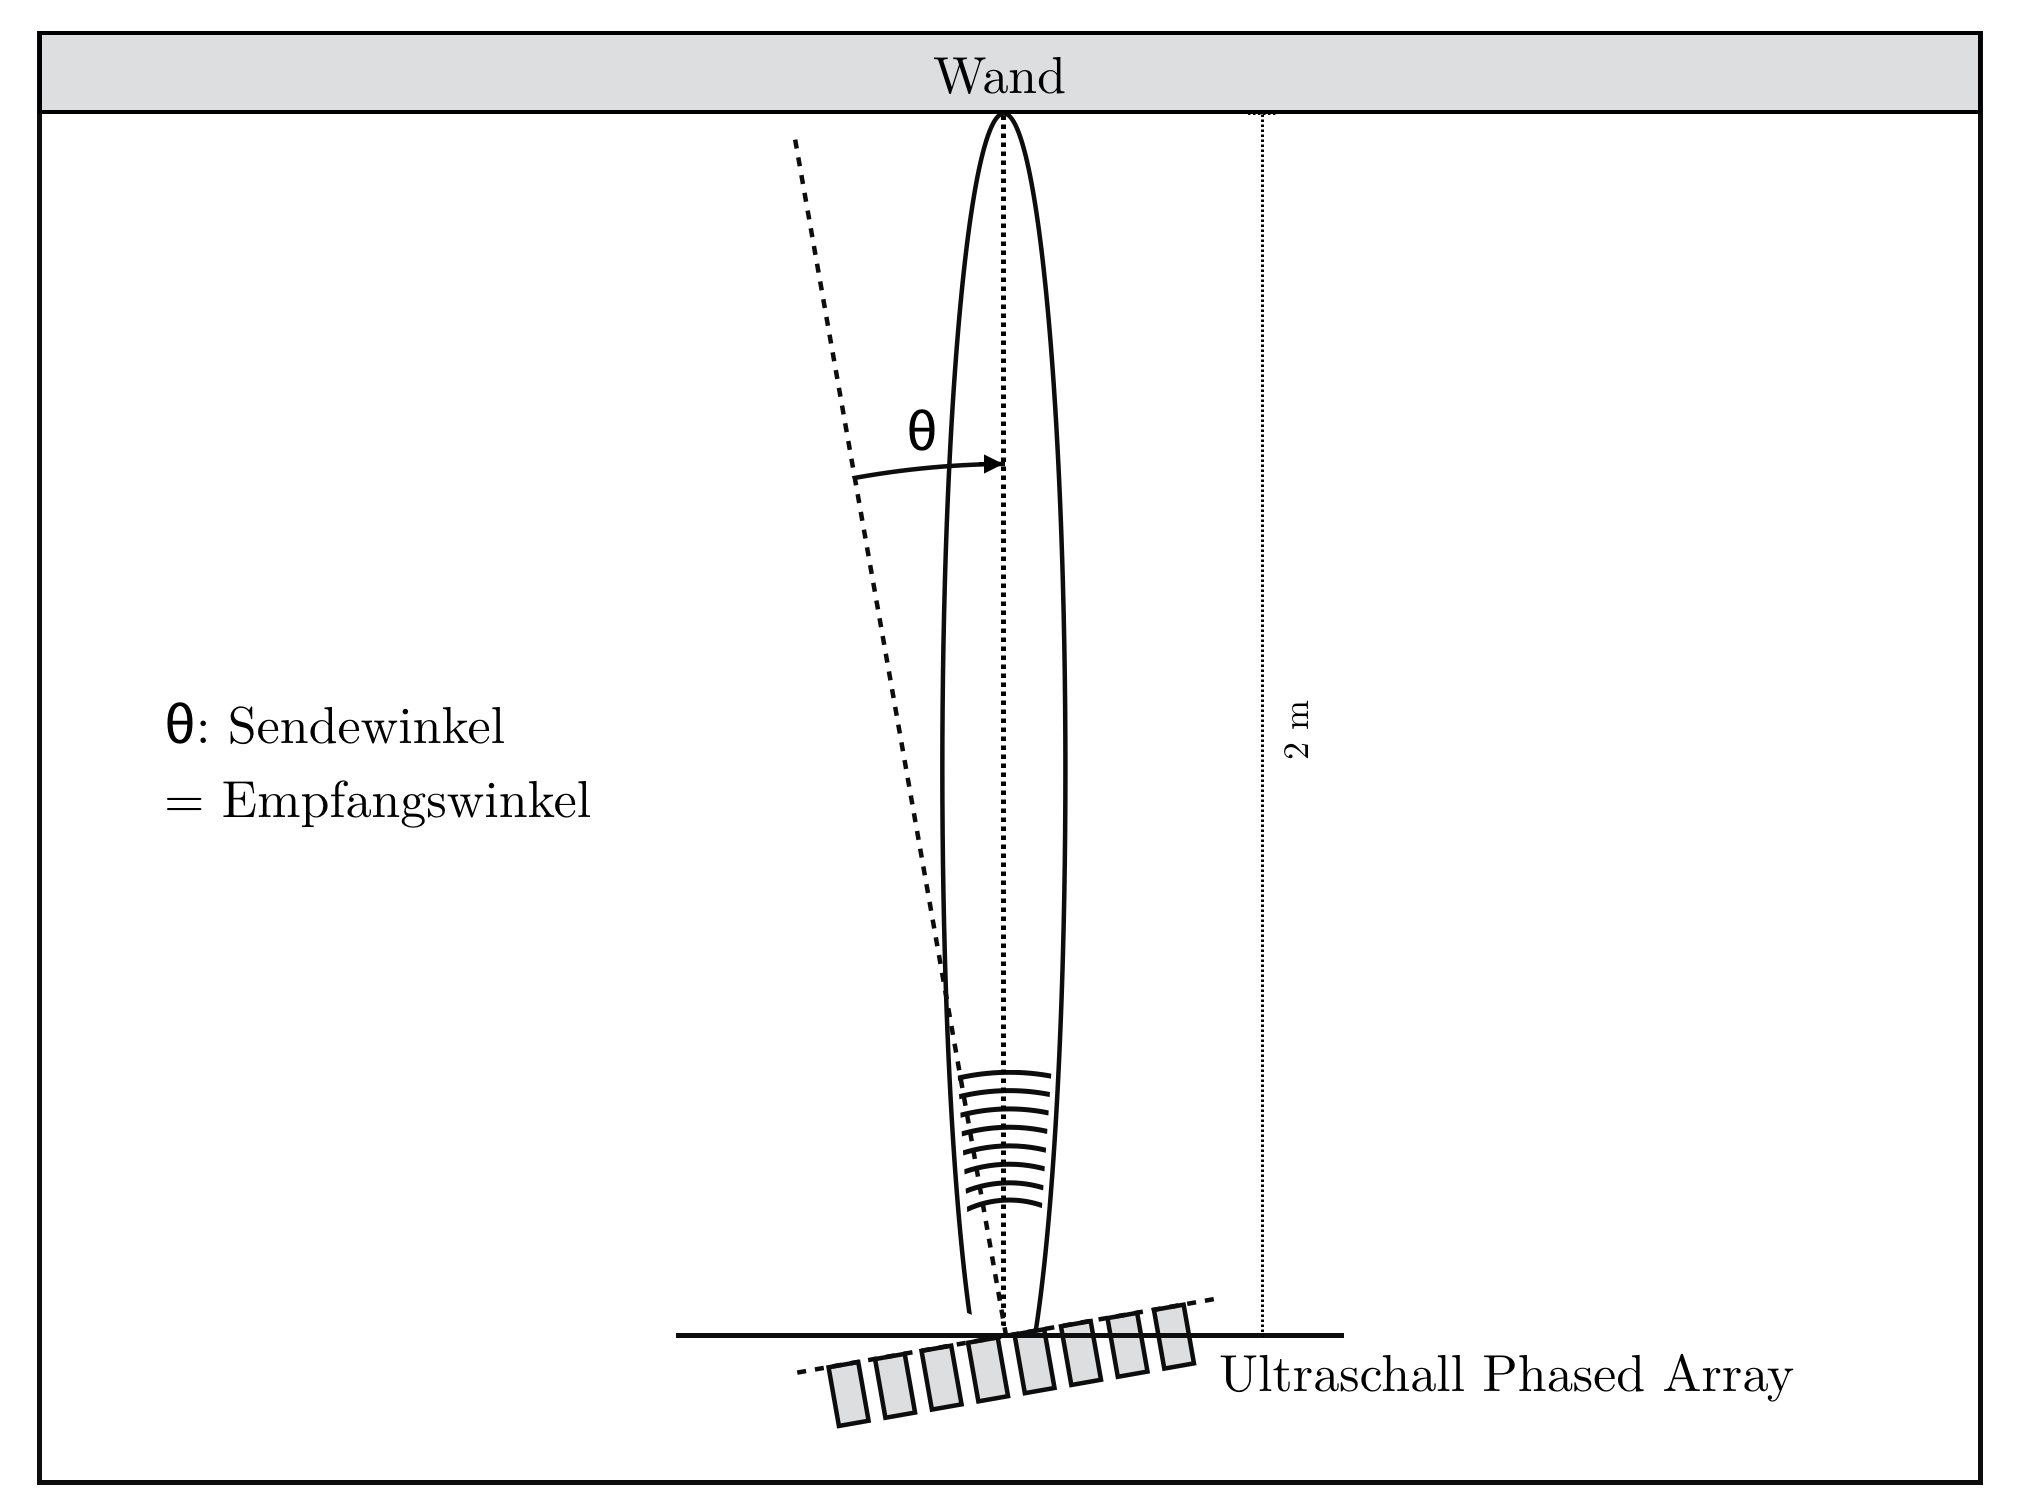
\includegraphics[width=\textwidth]{graphics/image_test_messaufbau_1.png}
\caption{Messaufbau zur empfangsseitigen Richtcharakteristik} % picture caption
\label{fig:image_test_messaufbau_1}
\end{figure}
%
%(Abb. \ref{fig:image1})
%%%%%%%%%%%%%%%%%%%%%%%%%%%%%%%%%%%%%%%%%%%%%%%%%%%%%%%%%%%%%%%%%%%%%%%%%%%%%%%%

\clearpage

\subsubsection{Messung der Empfangscharakteristik bei einem Sendewinkel von 0 Grad}
Das Gerät wird mithilfe des Heatmap-Graphen im GUI in einer Distanz von $2 \mathrm{m}$ für einen Sendewinkel von $\theta = 0^{\circ}$ senkrecht auf eine Wand ausgerichtet. Ein Umgebungsscan der Messsituation ist dabei in Abbildung \ref{fig:image_test_characteristic_receiver_0_deg_send} zu sehen. Es werden für die Messung vier Sendepulse ausgesandt.

%%%%%%%%%%%%%%%%%%%%%%%%%%%%%%%%%%%%%%%%%%%%%%%%%%%%%%%%%%%%%%%%%%%%%%%%%%%%%%%%
% pictures
\begin{figure}[htb]
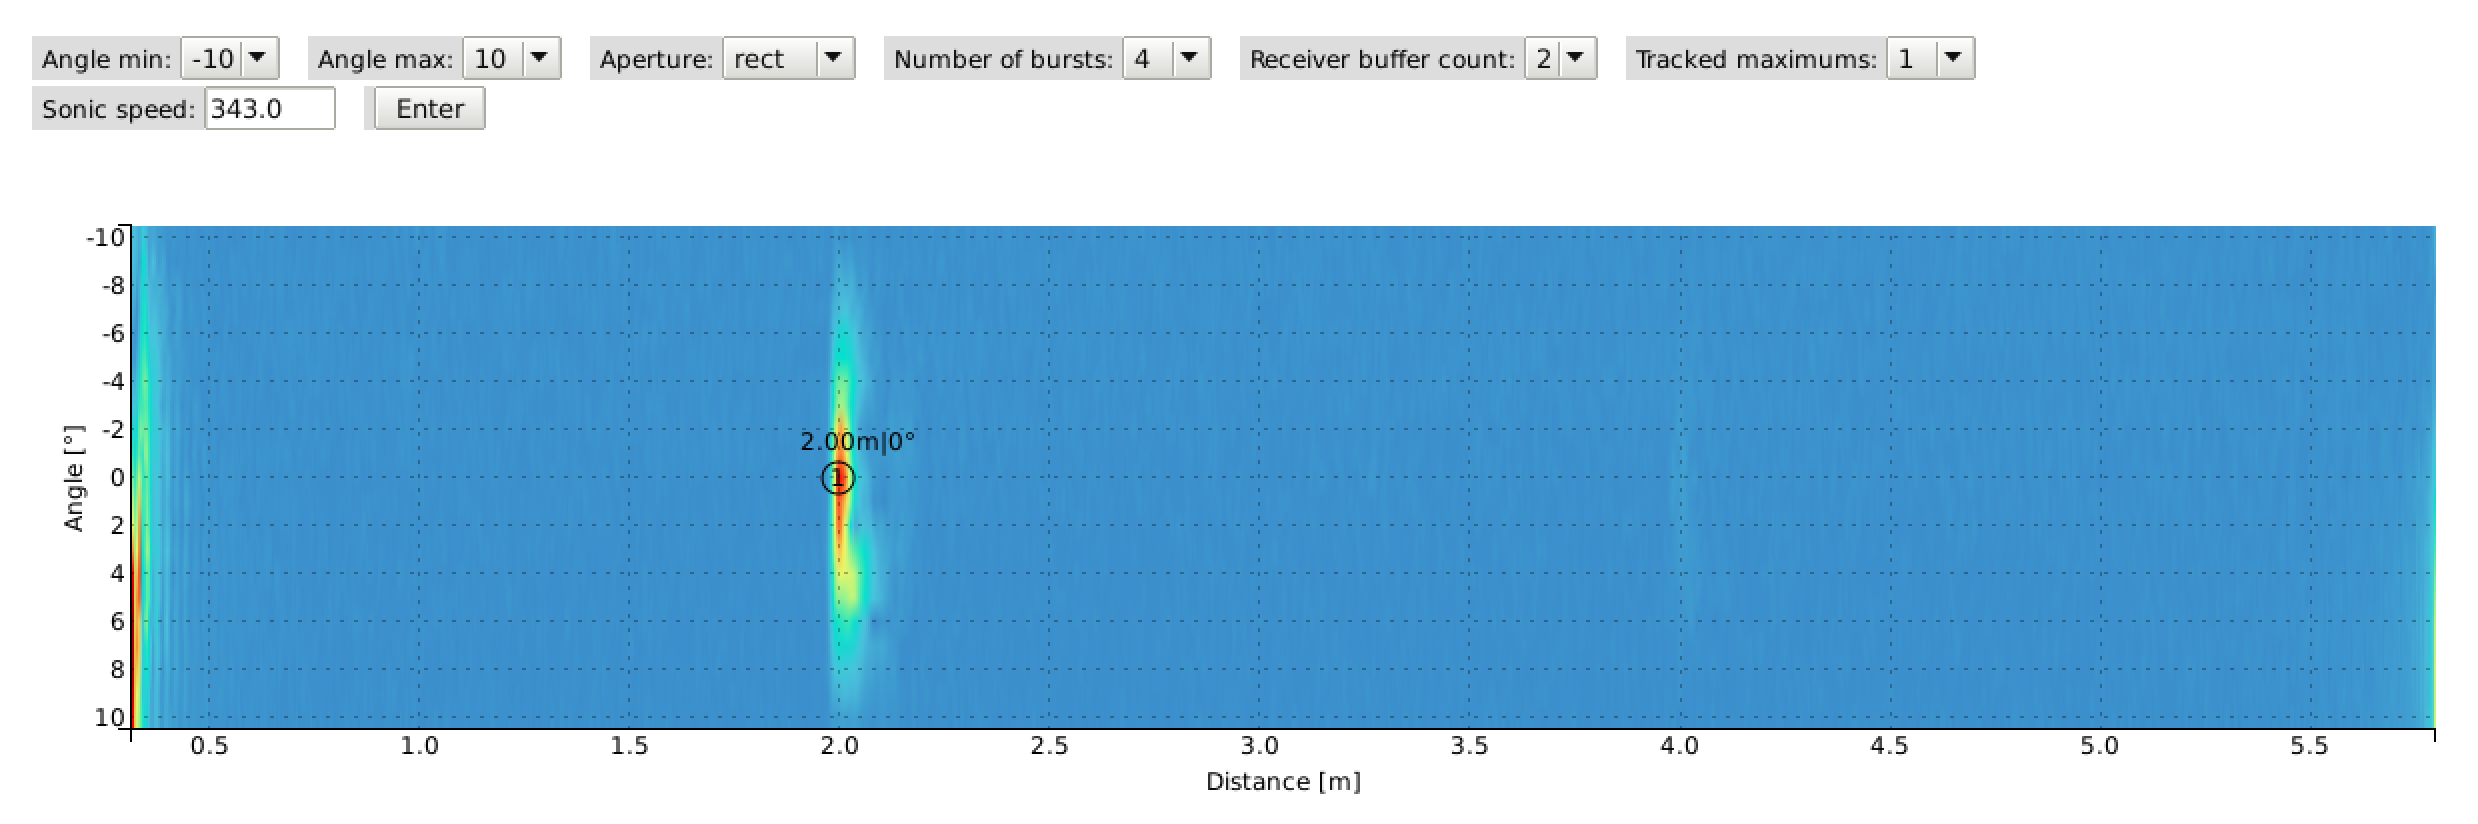
\includegraphics[width=\textwidth]{graphics/image_test_characteristic_receiver_0_deg_send.png}
\caption{Maximum bei $2.00 \mathrm{m}$ und $0^{\circ}$} % picture caption
\label{fig:image_test_characteristic_receiver_0_deg_send}
\end{figure}
%
%(Abb. \ref{fig:image1})
%%%%%%%%%%%%%%%%%%%%%%%%%%%%%%%%%%%%%%%%%%%%%%%%%%%%%%%%%%%%%%%%%%%%%%%%%%%%%%%%

Es entstehen dabei die Abbildungen \ref{fig:plot_test_characteristic_receiver_0_deg_send_rect_receive_rect_4_bursts}, \ref{fig:plot_test_characteristic_receiver_0_deg_send_rect_receive_cos_4_bursts}, \ref{fig:plot_test_characteristic_receiver_0_deg_send_rect_receive_cos2_4_bursts} und \ref{fig:plot_test_characteristic_receiver_0_deg_send_rect_receive_gauss_4_bursts} mit den entsprechenden Amplitudenbelegungen.

Die empfangsseitige Richtcharakteristik stimmt dabei insgesamt gut mit der Theorie überein. Für die Hauptkeulen ist die Übereinstimmung sogar sehr gut. Es fällt jedoch auf, dass für die Belegungen erneut grössere Nebenkeulen vorhanden sind (siehe Kapitel \ref{sec:messung_der_sendeseitigen_richtcharakteristik_mit_amplitudenbelegung}), als theoretisch berechnet. Mögliche Gründe sind wieder mechanische Kopplung und/oder kleinere mechanische Ungenauigkeiten beim Auflöten.

Bei den ersten Nebenkeulen ist erkennbar, dass die Linke jeweils grösser ist als die Rechte. Dieses asymmetrische Verhalten ist ausgeprägter bei den Messungen mit Amplitudenbelegung (Abbildungen \ref{fig:plot_test_characteristic_receiver_0_deg_send_rect_receive_cos_4_bursts}, \ref{fig:plot_test_characteristic_receiver_0_deg_send_rect_receive_cos2_4_bursts} und \ref{fig:plot_test_characteristic_receiver_0_deg_send_rect_receive_gauss_4_bursts}).

Desweiteren ist zu erkennen, dass das Ultraschall Phased Array zwar nicht mit genau $0^{\circ}$ senden kann (siehe Kapitel \ref{sec:messung_der_sendeseitigen_richtcharakteristik}), jedoch mit $0^{\circ}$ empfangen kann. Im Gegensatz zur Verzögerung beim Einschalten der PWM-Kanäle kann der Fehler, der durch das ADC-Multiplexing entsteht (siehe Kapitel \ref{sec:multiplexing}) im Nachhinein korrigiert werden.

\clearpage
\begin{figure}[htb]
\begin{minipage}{0.5\textwidth}
%%%%%%%%%%%%%%%%%%%%%%%%%%%%%%%%%%%%%%%%%%%%%%%%%%%%%%%%%%%%%%%%%%%%%%%%%%%%%%%%
% pictures
%\begin{figure}[htb]
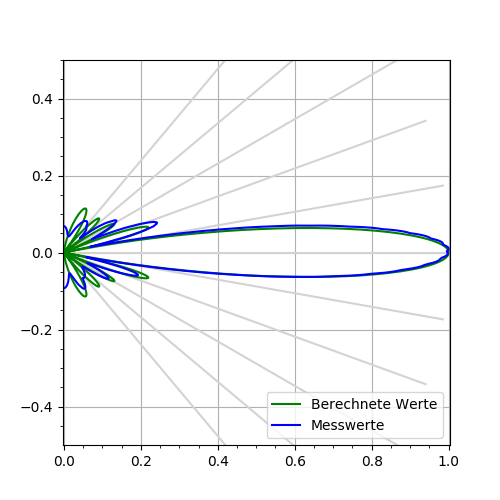
\includegraphics[width=\textwidth]{graphics/plot_test_characteristic_receiver_0_deg_send_rect_receive_rect_4_bursts.png}
\caption{Richtcharakteristik des Empfangs-Arrays für eine rechteckige Amplitudenbelegung} % picture caption
\label{fig:plot_test_characteristic_receiver_0_deg_send_rect_receive_rect_4_bursts}
%\end{figure}
%
%(Abb. \ref{fig:image1})
%%%%%%%%%%%%%%%%%%%%%%%%%%%%%%%%%%%%%%%%%%%%%%%%%%%%%%%%%%%%%%%%%%%%%%%%%%%%%%%%
\end{minipage}
\begin{minipage}{0.5\textwidth}
%%%%%%%%%%%%%%%%%%%%%%%%%%%%%%%%%%%%%%%%%%%%%%%%%%%%%%%%%%%%%%%%%%%%%%%%%%%%%%%%
% pictures
%\begin{figure}[htb]
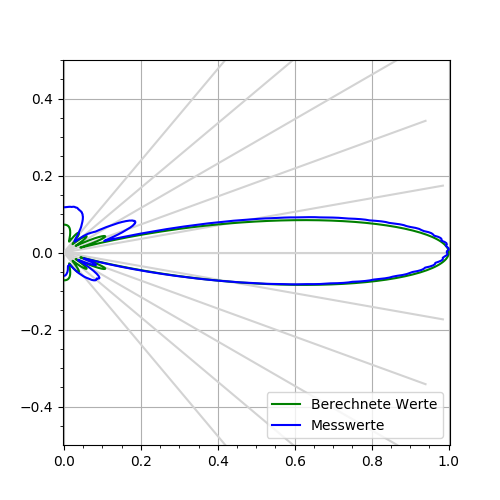
\includegraphics[width=\textwidth]{graphics/plot_test_characteristic_receiver_0_deg_send_rect_receive_cos_4_bursts.png}
\caption{Richtcharakteristik des Empfangs-Arrays für eine $\cos$-förmige Amplitudenbelegung} % picture caption
\label{fig:plot_test_characteristic_receiver_0_deg_send_rect_receive_cos_4_bursts}
%\end{figure}
%
%(Abb. \ref{fig:image1})
%%%%%%%%%%%%%%%%%%%%%%%%%%%%%%%%%%%%%%%%%%%%%%%%%%%%%%%%%%%%%%%%%%%%%%%%%%%%%%%%
\end{minipage}
\begin{minipage}{0.5\textwidth}
%%%%%%%%%%%%%%%%%%%%%%%%%%%%%%%%%%%%%%%%%%%%%%%%%%%%%%%%%%%%%%%%%%%%%%%%%%%%%%%%
% pictures
%\begin{figure}[htb]
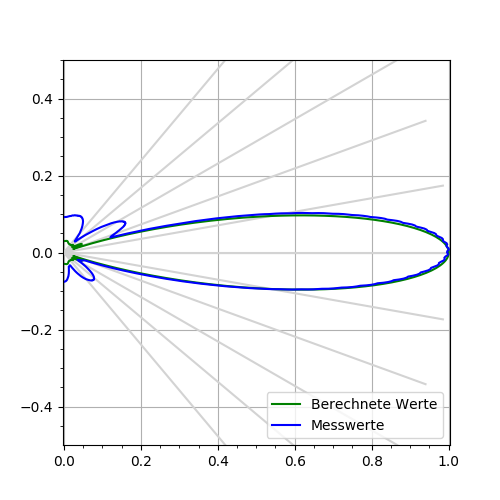
\includegraphics[width=\textwidth]{graphics/plot_test_characteristic_receiver_0_deg_send_rect_receive_cos2_4_bursts.png}
\caption{Richtcharakteristik des Empfangs-Arrays für eine $\cos^{2}$-förmige Amplitudenbelegung} % picture caption
\label{fig:plot_test_characteristic_receiver_0_deg_send_rect_receive_cos2_4_bursts}
%\end{figure}
%
%(Abb. \ref{fig:image1})
%%%%%%%%%%%%%%%%%%%%%%%%%%%%%%%%%%%%%%%%%%%%%%%%%%%%%%%%%%%%%%%%%%%%%%%%%%%%%%%%
\end{minipage}
\begin{minipage}{0.5\textwidth}
%%%%%%%%%%%%%%%%%%%%%%%%%%%%%%%%%%%%%%%%%%%%%%%%%%%%%%%%%%%%%%%%%%%%%%%%%%%%%%%%
% pictures
%\begin{figure}[htb]
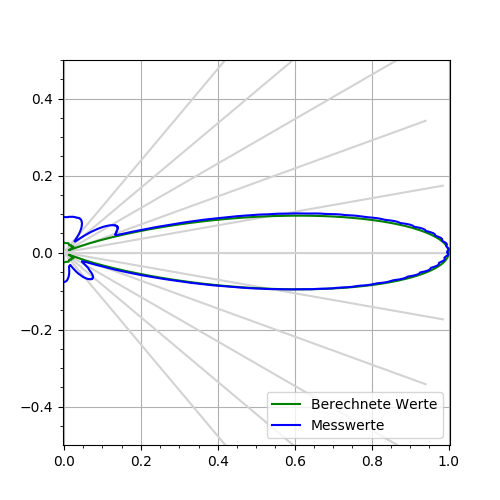
\includegraphics[width=\textwidth]{graphics/plot_test_characteristic_receiver_0_deg_send_rect_receive_gauss_4_bursts.png}
\caption{Richtcharakteristik des Empfangs-Arrays für eine gaussförmige Amplitudenbelegung} % picture caption
\label{fig:plot_test_characteristic_receiver_0_deg_send_rect_receive_gauss_4_bursts}
%\end{figure}
%
%(Abb. \ref{fig:image1})
%%%%%%%%%%%%%%%%%%%%%%%%%%%%%%%%%%%%%%%%%%%%%%%%%%%%%%%%%%%%%%%%%%%%%%%%%%%%%%%%
\end{minipage}
\end{figure}

\clearpage


\subsubsection{Messung der Empfangscharakteristik bei einem Sendewinkel von 10 Grad}
Mithilfe des Heatmap-Graphen im GUI wird das Gerät in $2 \mathrm{m}$ Distanz für einen Sendewinkel von $\theta = 10^{\circ}$ senkrecht auf eine Wand ausgerichtet. Die Messsituation ist dabei als Umgebungsscan in Abbildung \ref{fig:image_test_characteristic_receiver_0_deg_send} dargestellt. Zur Erzeugung des Sendesignals werden vier Sendepulse ausgesandt.

%%%%%%%%%%%%%%%%%%%%%%%%%%%%%%%%%%%%%%%%%%%%%%%%%%%%%%%%%%%%%%%%%%%%%%%%%%%%%%%%
% pictures
\begin{figure}[htb]
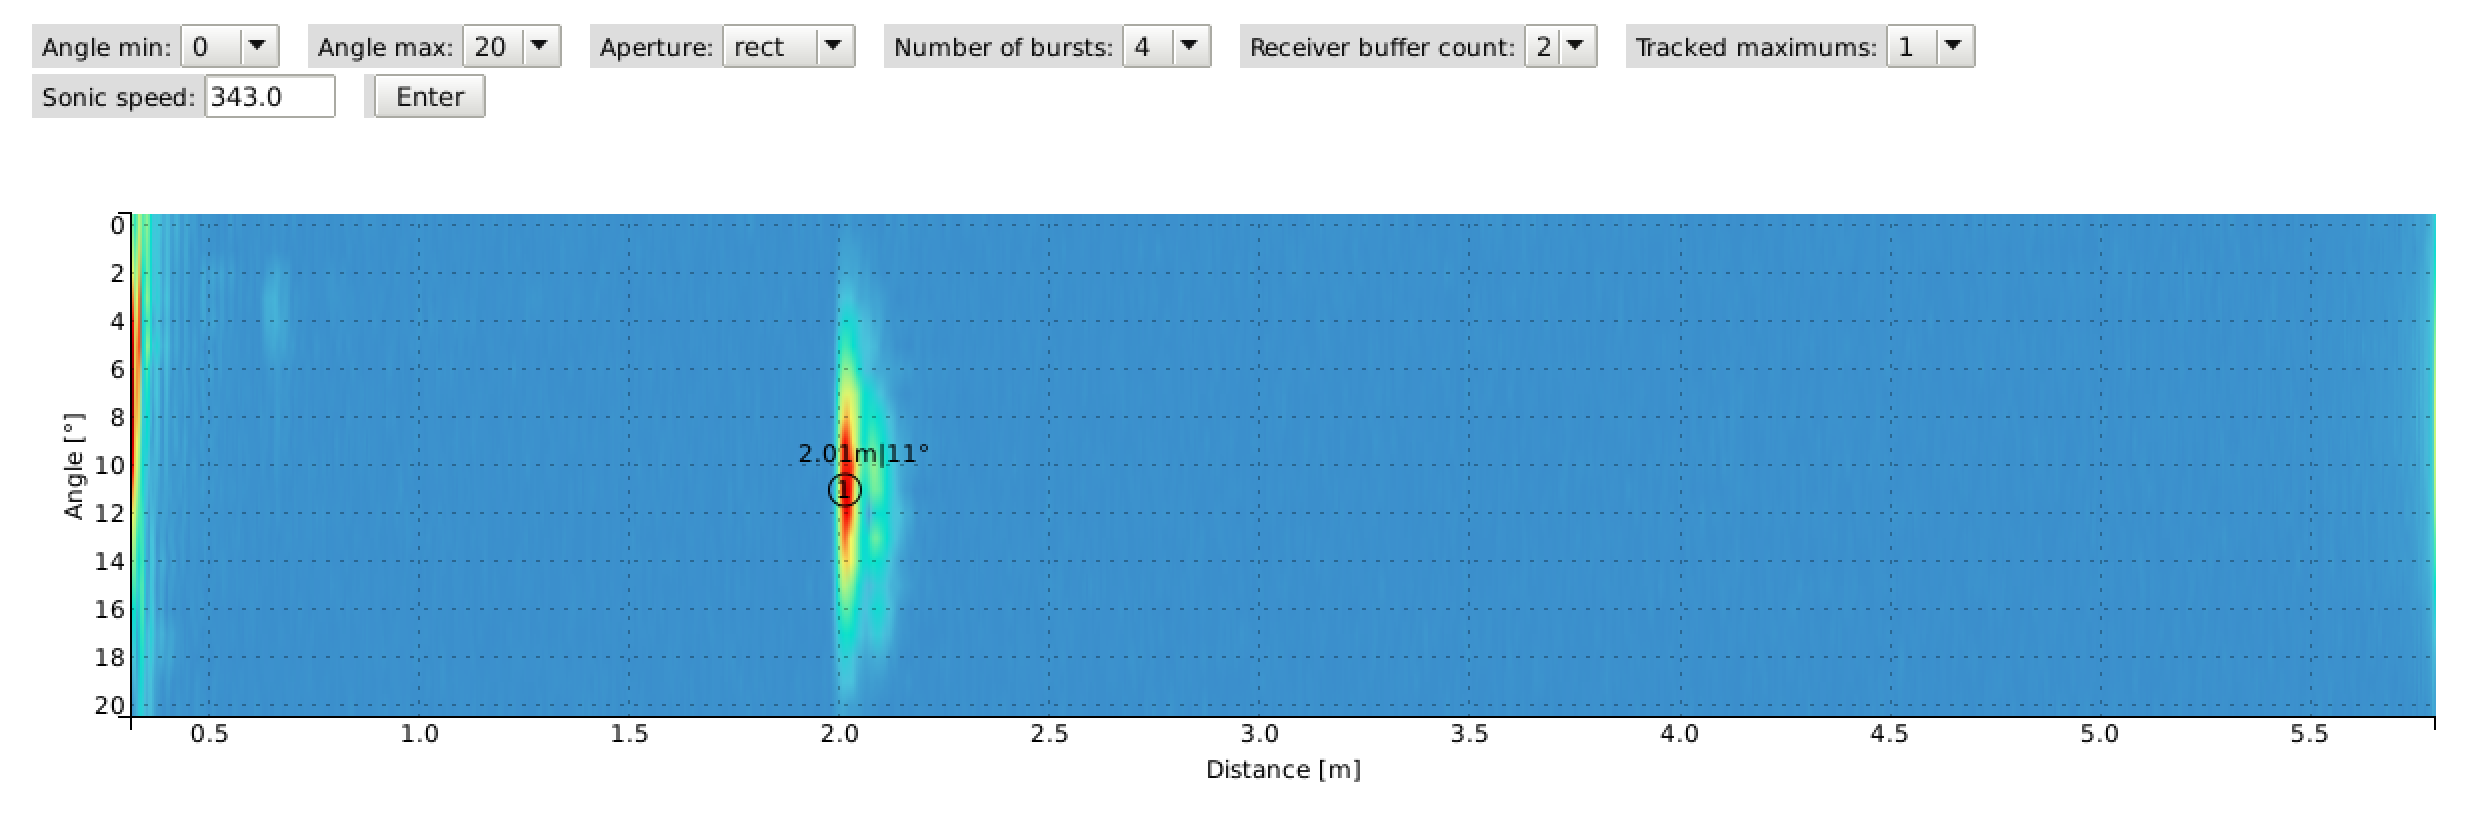
\includegraphics[width=\textwidth]{graphics/image_test_characteristic_receiver_10_deg_send.png}
\caption{Maximum bei $2.01 \mathrm{m}$ und $11^{\circ}$} % picture caption
\label{fig:image_test_characteristic_receiver_10_deg_send}
\end{figure}
%
%(Abb. \ref{fig:image1})
%%%%%%%%%%%%%%%%%%%%%%%%%%%%%%%%%%%%%%%%%%%%%%%%%%%%%%%%%%%%%%%%%%%%%%%%%%%%%%%%

Dabei entstehen die Abbildungen \ref{fig:plot_test_characteristic_receiver_10_deg_send_rect_receive_rect_4_bursts}, \ref{fig:plot_test_characteristic_receiver_10_deg_send_rect_receive_cos_4_bursts}, \ref{fig:plot_test_characteristic_receiver_10_deg_send_rect_receive_cos2_4_bursts} und \ref{fig:plot_test_characteristic_receiver_10_deg_send_rect_receive_gauss_4_bursts} mit den entsprechenden Amplitudenbelegungen.

Theorie und Messungen stimmen insgesamt wieder gut überein. Die Hauptkeulen sind dabei etwas breiter als berechnet und weisen einen Winkeloffset von ein paar Grad in negativer Richtung auf.

Wieder treten etwas grössere Nebenkeulen auf, als theoretisch berechnet. In Abbildung \ref{fig:plot_test_characteristic_receiver_10_deg_send_rect_receive_cos2_4_bursts} ist erneut erkennbar, wie die erste Nebenkeule links etwas grösser ist als auf der rechten Seite.

\clearpage
\begin{figure}[htb]
\begin{minipage}{0.5\textwidth}
%%%%%%%%%%%%%%%%%%%%%%%%%%%%%%%%%%%%%%%%%%%%%%%%%%%%%%%%%%%%%%%%%%%%%%%%%%%%%%%%
% pictures
%\begin{figure}[htb]
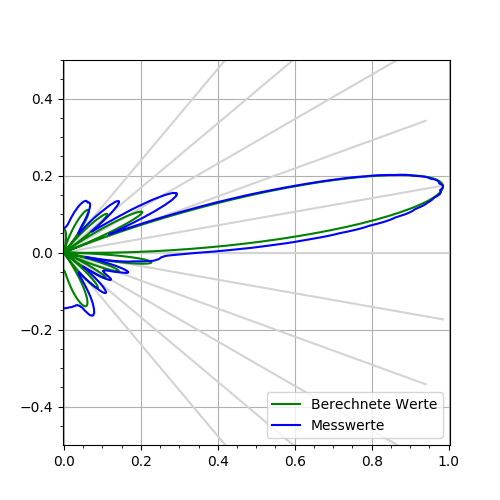
\includegraphics[width=\textwidth]{graphics/plot_test_characteristic_receiver_10_deg_send_rect_receive_rect_4_bursts.png}
\caption{Richtcharakteristik des Empfangs-Arrays für eine rechteckige Amplitudenbelegung} % picture caption
\label{fig:plot_test_characteristic_receiver_10_deg_send_rect_receive_rect_4_bursts}
%\end{figure}
%
%(Abb. \ref{fig:image1})
%%%%%%%%%%%%%%%%%%%%%%%%%%%%%%%%%%%%%%%%%%%%%%%%%%%%%%%%%%%%%%%%%%%%%%%%%%%%%%%%
\end{minipage}
\begin{minipage}{0.5\textwidth}
%%%%%%%%%%%%%%%%%%%%%%%%%%%%%%%%%%%%%%%%%%%%%%%%%%%%%%%%%%%%%%%%%%%%%%%%%%%%%%%%
% pictures
%\begin{figure}[htb]
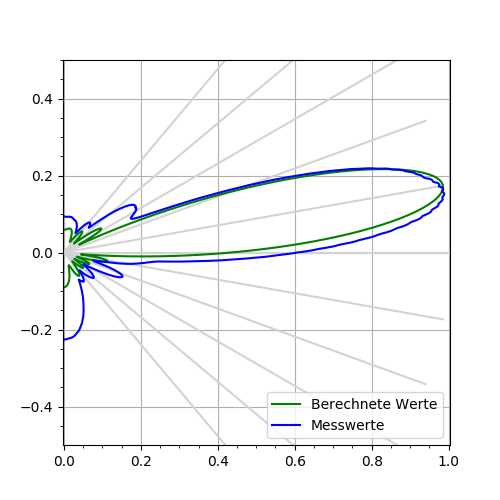
\includegraphics[width=\textwidth]{graphics/plot_test_characteristic_receiver_10_deg_send_rect_receive_cos_4_bursts.png}
\caption{Richtcharakteristik des Empfangs-Arrays für eine $\cos$-förmige Amplitudenbelegung} % picture caption
\label{fig:plot_test_characteristic_receiver_10_deg_send_rect_receive_cos_4_bursts}
%\end{figure}
%
%(Abb. \ref{fig:image1})
%%%%%%%%%%%%%%%%%%%%%%%%%%%%%%%%%%%%%%%%%%%%%%%%%%%%%%%%%%%%%%%%%%%%%%%%%%%%%%%%
\end{minipage}
\begin{minipage}{0.5\textwidth}
%%%%%%%%%%%%%%%%%%%%%%%%%%%%%%%%%%%%%%%%%%%%%%%%%%%%%%%%%%%%%%%%%%%%%%%%%%%%%%%%
% pictures
%\begin{figure}[htb]
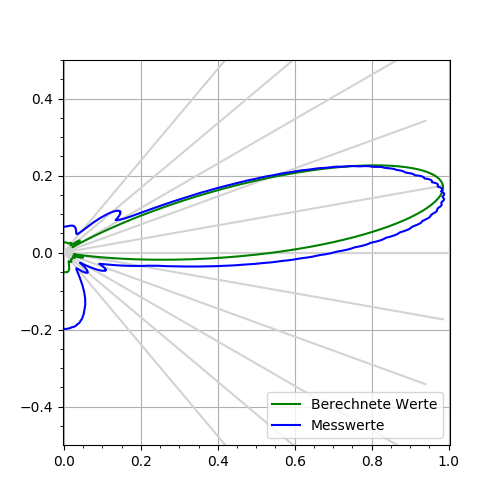
\includegraphics[width=\textwidth]{graphics/plot_test_characteristic_receiver_10_deg_send_rect_receive_cos2_4_bursts.png}
\caption{Richtcharakteristik des Empfangs-Arrays für eine $\cos^{2}$-förmige Amplitudenbelegung} % picture caption
\label{fig:plot_test_characteristic_receiver_10_deg_send_rect_receive_cos2_4_bursts}
%\end{figure}
%
%(Abb. \ref{fig:image1})
%%%%%%%%%%%%%%%%%%%%%%%%%%%%%%%%%%%%%%%%%%%%%%%%%%%%%%%%%%%%%%%%%%%%%%%%%%%%%%%%
\end{minipage}
\begin{minipage}{0.5\textwidth}
%%%%%%%%%%%%%%%%%%%%%%%%%%%%%%%%%%%%%%%%%%%%%%%%%%%%%%%%%%%%%%%%%%%%%%%%%%%%%%%%
% pictures
%\begin{figure}[htb]
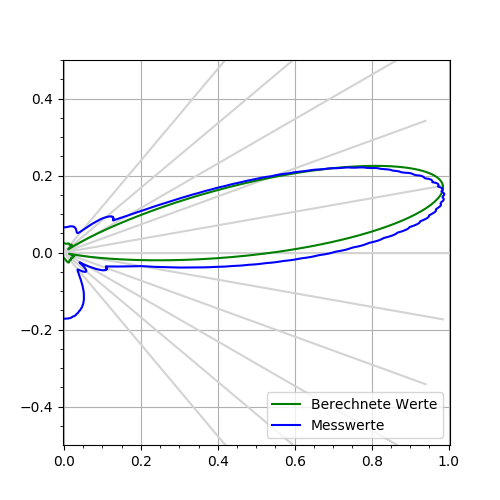
\includegraphics[width=\textwidth]{graphics/plot_test_characteristic_receiver_10_deg_send_rect_receive_gauss_4_bursts.png}
\caption{Richtcharakteristik des Empfangs-Arrays für eine gaussförmige Amplitudenbelegung} % picture caption
\label{fig:plot_test_characteristic_receiver_10_deg_send_rect_receive_gauss_4_bursts}
%\end{figure}
%
%(Abb. \ref{fig:image1})
%%%%%%%%%%%%%%%%%%%%%%%%%%%%%%%%%%%%%%%%%%%%%%%%%%%%%%%%%%%%%%%%%%%%%%%%%%%%%%%%
\end{minipage}
\end{figure}

\clearpage


\subsubsection{Messung der Empfangscharakteristik bei einem Sendewinkel von 20 Grad}
Über den Heatmap-Graph im GUI wird das Gerät in $2 \mathrm{m}$ Distanz für einen Sendewinkel von $\theta = 20^{\circ}$ senkrecht auf eine Wand ausgerichtet. Ein Umgebungsscan der Messsituation ist in Abbildung \ref{fig:image_test_characteristic_receiver_0_deg_send} dargestellt. Für die Messung werden vier Sendepulse ausgesandt.

%%%%%%%%%%%%%%%%%%%%%%%%%%%%%%%%%%%%%%%%%%%%%%%%%%%%%%%%%%%%%%%%%%%%%%%%%%%%%%%%
% pictures
\begin{figure}[htb]
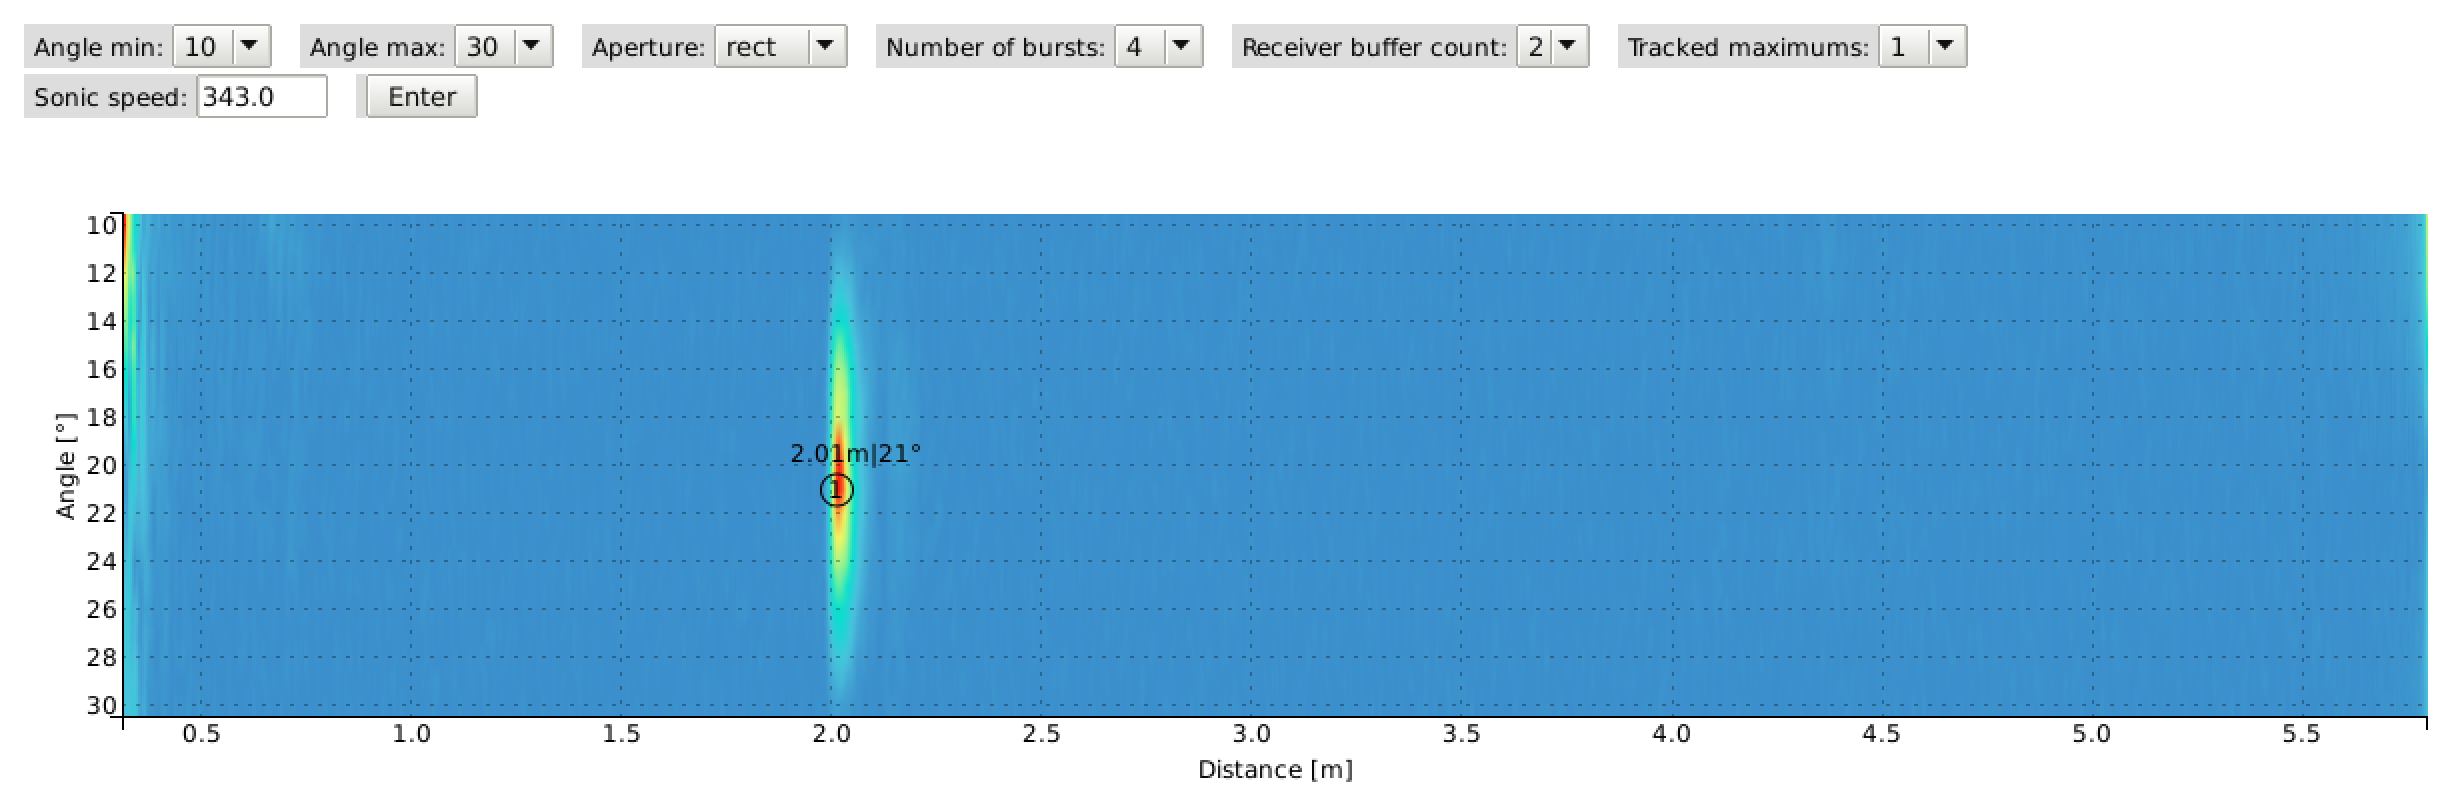
\includegraphics[width=\textwidth]{graphics/image_test_characteristic_receiver_20_deg_send.png}
\caption{Maximum bei $2.01 \mathrm{m}$ und $21^{\circ}$} % picture caption
\label{fig:image_test_characteristic_receiver_20_deg_send}
\end{figure}
%
%(Abb. \ref{fig:image1})
%%%%%%%%%%%%%%%%%%%%%%%%%%%%%%%%%%%%%%%%%%%%%%%%%%%%%%%%%%%%%%%%%%%%%%%%%%%%%%%%

Das Ergebnis wird in den Abbildungen \ref{fig:plot_test_characteristic_receiver_20_deg_send_rect_receive_rect_4_bursts}, \ref{fig:plot_test_characteristic_receiver_20_deg_send_rect_receive_cos_4_bursts}, \ref{fig:plot_test_characteristic_receiver_20_deg_send_rect_receive_cos2_4_bursts} und \ref{fig:plot_test_characteristic_receiver_20_deg_send_rect_receive_gauss_4_bursts} mit den entsprechenden Amplitudenbelegungen dargestellt.

Erneut stimmen Theorie und Messungen gut überein. Die Hauptkeule ist nahezu identisch zum berechneten Verlauf.

Wie bei den vorherigen Messreihen treten für die Belegungen grössere Nebenkeulen auf als berechnet. In den Abbildungen \ref{fig:plot_test_characteristic_receiver_20_deg_send_rect_receive_cos2_4_bursts} und \ref{fig:plot_test_characteristic_receiver_20_deg_send_rect_receive_gauss_4_bursts} ist dies gut erkennbar. Wie bereits erwähnt, könnten die grösseren Nebenkeulen auf mechanische Kopplung und/oder mechanische Ungenauigkeiten beim Auflöten zurückzuführen sein. Die Asymmetrie zwischen den links- und rechtsseitigen Nebenkeulen ist jedoch weniger ausgeprägt als in den vorherigen Messreihen.

\clearpage
\begin{figure}[htb]
\begin{minipage}{0.5\textwidth}
%%%%%%%%%%%%%%%%%%%%%%%%%%%%%%%%%%%%%%%%%%%%%%%%%%%%%%%%%%%%%%%%%%%%%%%%%%%%%%%%
% pictures
%\begin{figure}[htb]
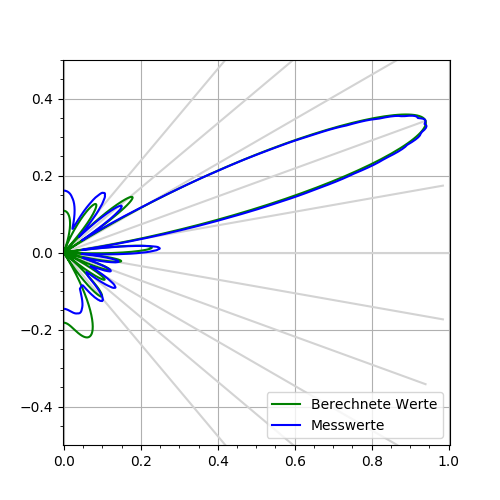
\includegraphics[width=\textwidth]{graphics/plot_test_characteristic_receiver_20_deg_send_rect_receive_rect_4_bursts.png}
\caption{Richtcharakteristik des Empfangs-Arrays für eine rechteckige Amplitudenbelegung} % picture caption
\label{fig:plot_test_characteristic_receiver_20_deg_send_rect_receive_rect_4_bursts}
%\end{figure}
%
%(Abb. \ref{fig:image1})
%%%%%%%%%%%%%%%%%%%%%%%%%%%%%%%%%%%%%%%%%%%%%%%%%%%%%%%%%%%%%%%%%%%%%%%%%%%%%%%%
\end{minipage}
\begin{minipage}{0.5\textwidth}
%%%%%%%%%%%%%%%%%%%%%%%%%%%%%%%%%%%%%%%%%%%%%%%%%%%%%%%%%%%%%%%%%%%%%%%%%%%%%%%%
% pictures
%\begin{figure}[htb]
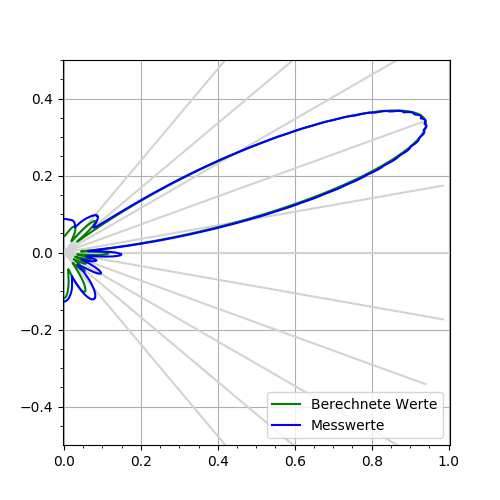
\includegraphics[width=\textwidth]{graphics/plot_test_characteristic_receiver_20_deg_send_rect_receive_cos_4_bursts.png}
\caption{Richtcharakteristik des Empfangs-Arrays für eine $\cos$-förmige Amplitudenbelegung} % picture caption
\label{fig:plot_test_characteristic_receiver_20_deg_send_rect_receive_cos_4_bursts}
%\end{figure}
%
%(Abb. \ref{fig:image1})
%%%%%%%%%%%%%%%%%%%%%%%%%%%%%%%%%%%%%%%%%%%%%%%%%%%%%%%%%%%%%%%%%%%%%%%%%%%%%%%%
\end{minipage}
\begin{minipage}{0.5\textwidth}
%%%%%%%%%%%%%%%%%%%%%%%%%%%%%%%%%%%%%%%%%%%%%%%%%%%%%%%%%%%%%%%%%%%%%%%%%%%%%%%%
% pictures
%\begin{figure}[htb]
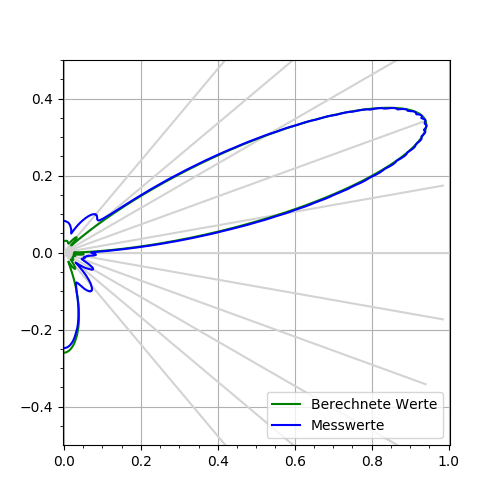
\includegraphics[width=\textwidth]{graphics/plot_test_characteristic_receiver_20_deg_send_rect_receive_cos2_4_bursts.png}
\caption{Richtcharakteristik des Empfangs-Arrays für eine $\cos^{2}$-förmige Amplitudenbelegung} % picture caption
\label{fig:plot_test_characteristic_receiver_20_deg_send_rect_receive_cos2_4_bursts}
%\end{figure}
%
%(Abb. \ref{fig:image1})
%%%%%%%%%%%%%%%%%%%%%%%%%%%%%%%%%%%%%%%%%%%%%%%%%%%%%%%%%%%%%%%%%%%%%%%%%%%%%%%%
\end{minipage}
\begin{minipage}{0.5\textwidth}
%%%%%%%%%%%%%%%%%%%%%%%%%%%%%%%%%%%%%%%%%%%%%%%%%%%%%%%%%%%%%%%%%%%%%%%%%%%%%%%%
% pictures
%\begin{figure}[htb]
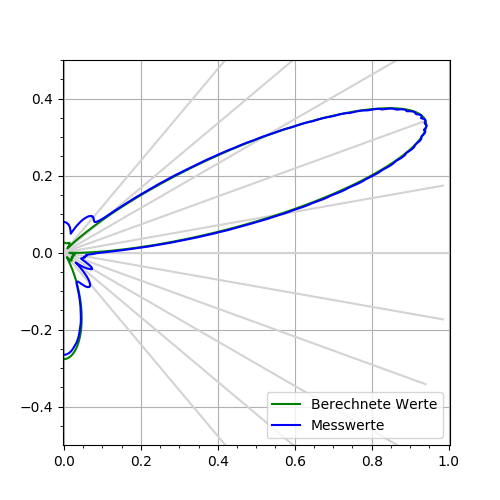
\includegraphics[width=\textwidth]{graphics/plot_test_characteristic_receiver_20_deg_send_rect_receive_gauss_4_bursts.png}
\caption{Richtcharakteristik des Empfangs-Arrays für eine gaussförmige Amplitudenbelegung} % picture caption
\label{fig:plot_test_characteristic_receiver_20_deg_send_rect_receive_gauss_4_bursts}
%\end{figure}
%
%(Abb. \ref{fig:image1})
%%%%%%%%%%%%%%%%%%%%%%%%%%%%%%%%%%%%%%%%%%%%%%%%%%%%%%%%%%%%%%%%%%%%%%%%%%%%%%%%
\end{minipage}
\end{figure}

\clearpage


\subsubsection{Messung der Empfangscharakteristik bei einem Sendewinkel von 30 Grad}
Mithilfe des Heatmap-Graphs im GUI wird das Gerät in $2 \mathrm{m}$ Distanz für einen Sendewinkel von $\theta = 30^{\circ}$ senkrecht auf eine Wand ausgerichtet. Die Messsituation ist dabei als Umgebungsscan in Abbildung \ref{fig:image_test_characteristic_receiver_0_deg_send} zu sehen. Das Sendesignal wird mit sechs Sendepulsen erzeugt.

%%%%%%%%%%%%%%%%%%%%%%%%%%%%%%%%%%%%%%%%%%%%%%%%%%%%%%%%%%%%%%%%%%%%%%%%%%%%%%%%
% pictures
\begin{figure}[htb]
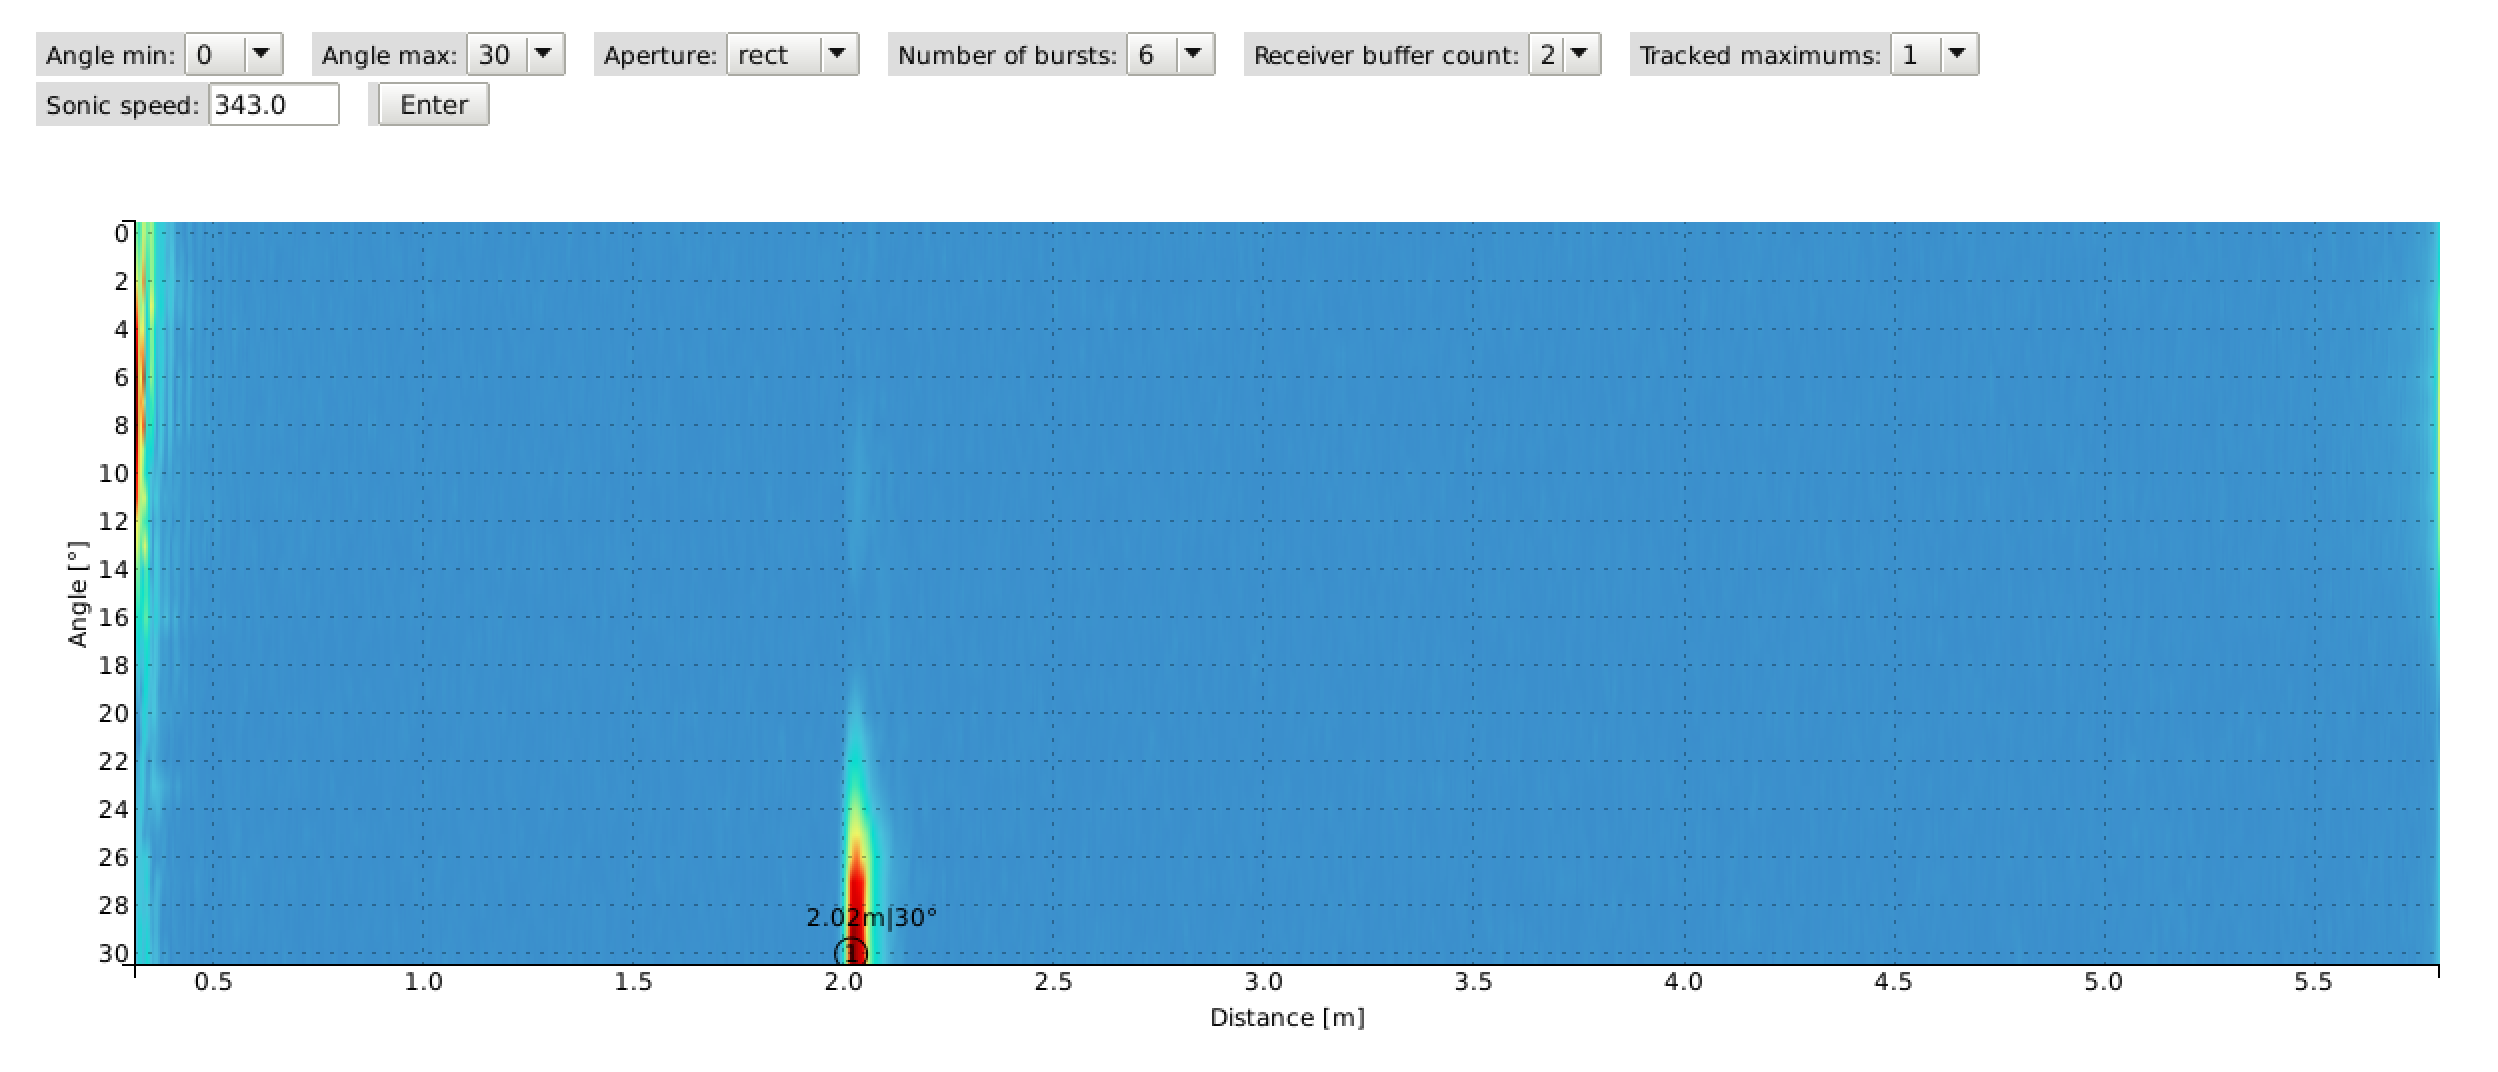
\includegraphics[width=\textwidth]{graphics/image_test_characteristic_receiver_30_deg_send.png}
\caption{Maximum bei $2.02 \mathrm{m}$ und $30^{\circ}$} % picture caption
\label{fig:image_test_characteristic_receiver_30_deg_send}
\end{figure}
%
%(Abb. \ref{fig:image1})
%%%%%%%%%%%%%%%%%%%%%%%%%%%%%%%%%%%%%%%%%%%%%%%%%%%%%%%%%%%%%%%%%%%%%%%%%%%%%%%%

Als Ergebnis entstehen dabei die Abbildungen \ref{fig:plot_test_characteristic_receiver_30_deg_send_rect_receive_rect_6_bursts}, \ref{fig:plot_test_characteristic_receiver_30_deg_send_rect_receive_cos_6_bursts}, \ref{fig:plot_test_characteristic_receiver_30_deg_send_rect_receive_cos2_6_bursts} und \ref{fig:plot_test_characteristic_receiver_30_deg_send_rect_receive_gauss_6_bursts} mit den entsprechenden Amplitudenbelegungen.

Theorie und Messungen stimmen insgesamt gut überein. Die Hauptkeule ist etwas breiter als berechnet und weist einen Winkeloffset von ein paar Grad in die positive Richtung auf.

Es fällt auf, dass im Gegensatz zu den vorherigen Messreihen für die Belegungen kaum grössere Nebenkeulen entstehen, als berechnet wurde. Dies ist in den Abbildungen \ref{fig:plot_test_characteristic_receiver_10_deg_send_rect_receive_cos2_4_bursts} und \ref{fig:plot_test_characteristic_receiver_10_deg_send_rect_receive_gauss_4_bursts} gut erkennbar.

Interessant ist, wie in Abbildung \ref{fig:plot_test_characteristic_receiver_30_deg_send_rect_receive_rect_6_bursts} die grosse Nebenkeule rechts aussen kleiner, in den Abbildungen \ref{fig:plot_test_characteristic_receiver_30_deg_send_rect_receive_cos_6_bursts}, \ref{fig:plot_test_characteristic_receiver_30_deg_send_rect_receive_cos2_6_bursts} und \ref{fig:plot_test_characteristic_receiver_30_deg_send_rect_receive_gauss_6_bursts} jedoch grösser ist als berechnet.

\clearpage
\begin{figure}[htb]
\begin{minipage}{0.5\textwidth}
%%%%%%%%%%%%%%%%%%%%%%%%%%%%%%%%%%%%%%%%%%%%%%%%%%%%%%%%%%%%%%%%%%%%%%%%%%%%%%%%
% pictures
%\begin{figure}[htb]
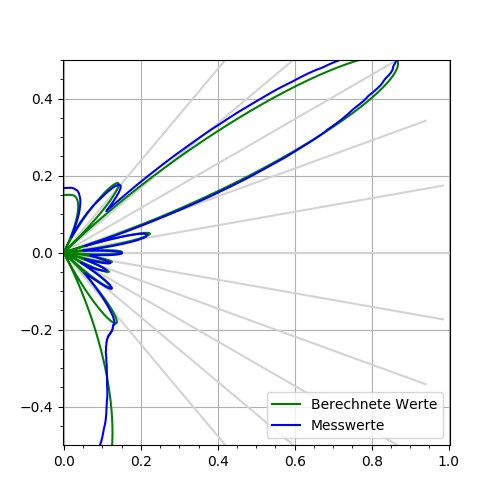
\includegraphics[width=\textwidth]{graphics/plot_test_characteristic_receiver_30_deg_send_rect_receive_rect_6_bursts.png}
\caption{Richtcharakteristik des Empfangs-Arrays für eine rechteckige Amplitudenbelegung} % picture caption
\label{fig:plot_test_characteristic_receiver_30_deg_send_rect_receive_rect_6_bursts}
%\end{figure}
%
%(Abb. \ref{fig:image1})
%%%%%%%%%%%%%%%%%%%%%%%%%%%%%%%%%%%%%%%%%%%%%%%%%%%%%%%%%%%%%%%%%%%%%%%%%%%%%%%%
\end{minipage}
\begin{minipage}{0.5\textwidth}
%%%%%%%%%%%%%%%%%%%%%%%%%%%%%%%%%%%%%%%%%%%%%%%%%%%%%%%%%%%%%%%%%%%%%%%%%%%%%%%%
% pictures
%\begin{figure}[htb]
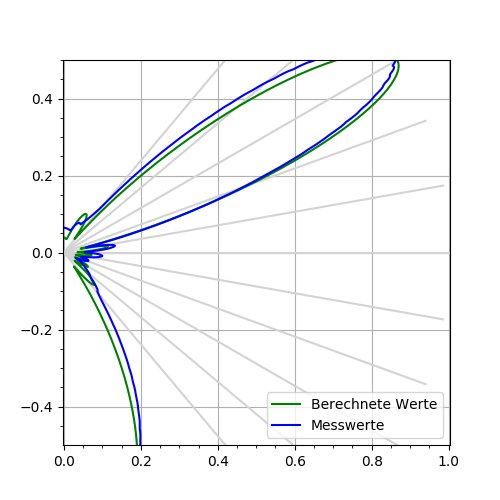
\includegraphics[width=\textwidth]{graphics/plot_test_characteristic_receiver_30_deg_send_rect_receive_cos_6_bursts.png}
\caption{Richtcharakteristik des Empfangs-Arrays für eine $\cos$-förmige Amplitudenbelegung} % picture caption
\label{fig:plot_test_characteristic_receiver_30_deg_send_rect_receive_cos_6_bursts}
%\end{figure}
%
%(Abb. \ref{fig:image1})
%%%%%%%%%%%%%%%%%%%%%%%%%%%%%%%%%%%%%%%%%%%%%%%%%%%%%%%%%%%%%%%%%%%%%%%%%%%%%%%%
\end{minipage}
\begin{minipage}{0.5\textwidth}
%%%%%%%%%%%%%%%%%%%%%%%%%%%%%%%%%%%%%%%%%%%%%%%%%%%%%%%%%%%%%%%%%%%%%%%%%%%%%%%%
% pictures
%\begin{figure}[htb]
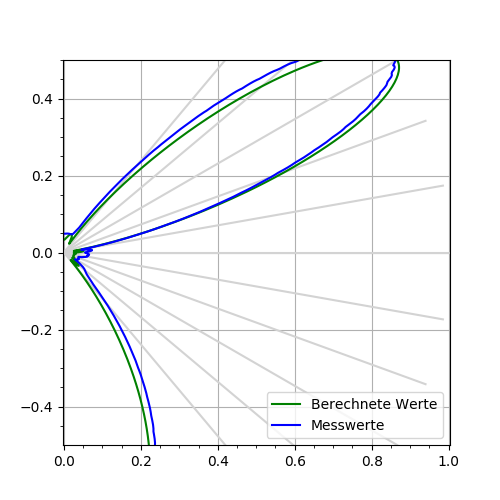
\includegraphics[width=\textwidth]{graphics/plot_test_characteristic_receiver_30_deg_send_rect_receive_cos2_6_bursts.png}
\caption{Richtcharakteristik des Empfangs-Arrays für eine $\cos^{2}$-förmige Amplitudenbelegung} % picture caption
\label{fig:plot_test_characteristic_receiver_30_deg_send_rect_receive_cos2_6_bursts}
%\end{figure}
%
%(Abb. \ref{fig:image1})
%%%%%%%%%%%%%%%%%%%%%%%%%%%%%%%%%%%%%%%%%%%%%%%%%%%%%%%%%%%%%%%%%%%%%%%%%%%%%%%%
\end{minipage}
\begin{minipage}{0.5\textwidth}
%%%%%%%%%%%%%%%%%%%%%%%%%%%%%%%%%%%%%%%%%%%%%%%%%%%%%%%%%%%%%%%%%%%%%%%%%%%%%%%%
% pictures
%\begin{figure}[htb]
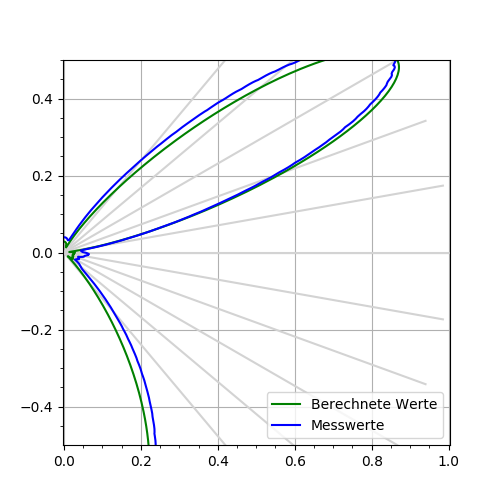
\includegraphics[width=\textwidth]{graphics/plot_test_characteristic_receiver_30_deg_send_rect_receive_gauss_6_bursts.png}
\caption{Richtcharakteristik des Empfangs-Arrays für eine gaussförmige Amplitudenbelegung} % picture caption
\label{fig:plot_test_characteristic_receiver_30_deg_send_rect_receive_gauss_6_bursts}
%\end{figure}
%
%(Abb. \ref{fig:image1})
%%%%%%%%%%%%%%%%%%%%%%%%%%%%%%%%%%%%%%%%%%%%%%%%%%%%%%%%%%%%%%%%%%%%%%%%%%%%%%%%
\end{minipage}
\end{figure}


\clearpage
%%%%%%%%%%%%%%%%%%%%%%%%%%%%%%%%%%%%%%%%%%%%%%%%%%%%%%%%%%%%%%%%%%%%%%%%%%%%%%%%
%%%%%%%%%%%%%%%%%%%%%%%%%%%%%%%%%%%%%%%%%%%%%%%%%%%%%%%%%%%%%%%%%%%%%%%%%%%%%%%%
%%%%%%%%%%%%%%%%%%%%%%%%%%%%%%%%%%%%%%%%%%%%%%%%%%%%%%%%%%%%%%%%%%%%%%%%%%%%%%%%
\subsection{Distanzmessungen}\label{sec:distanzmessungen}
Für die Messung der Distanzauflösung wird das Gerät frontal vor einer glatten Wand aufgestellt und die Distanz vom Ultraschall Phased Array zur Wand gemessen. Daraufhin wird dieser Referenzwert verglichen mit dem Distanzwert aus dem GUI, welcher mithilfe der Maximum-Tracking Funktion abgelesen wird. Die dadurch entstehen Umgebungsscans sind jeweils dargestellt. Störende Boden- und Deckenreflexionen werden mit einem Schaumstoffstück verhindert. Für grössere Distanzen wird aufgrund der Dämpfung die Anzahl Sendepulse erhöht. Für jede Messung ist die Anzahl Pulse vermerkt.

\begin{figure}[htb]
\begin{minipage}{1.0\textwidth}
%%%%%%%%%%%%%%%%%%%%%%%%%%%%%%%%%%%%%%%%%%%%%%%%%%%%%%%%%%%%%%%%%%%%%%%%%%%%%%%%
% pictures
%\begin{figure}[htb]
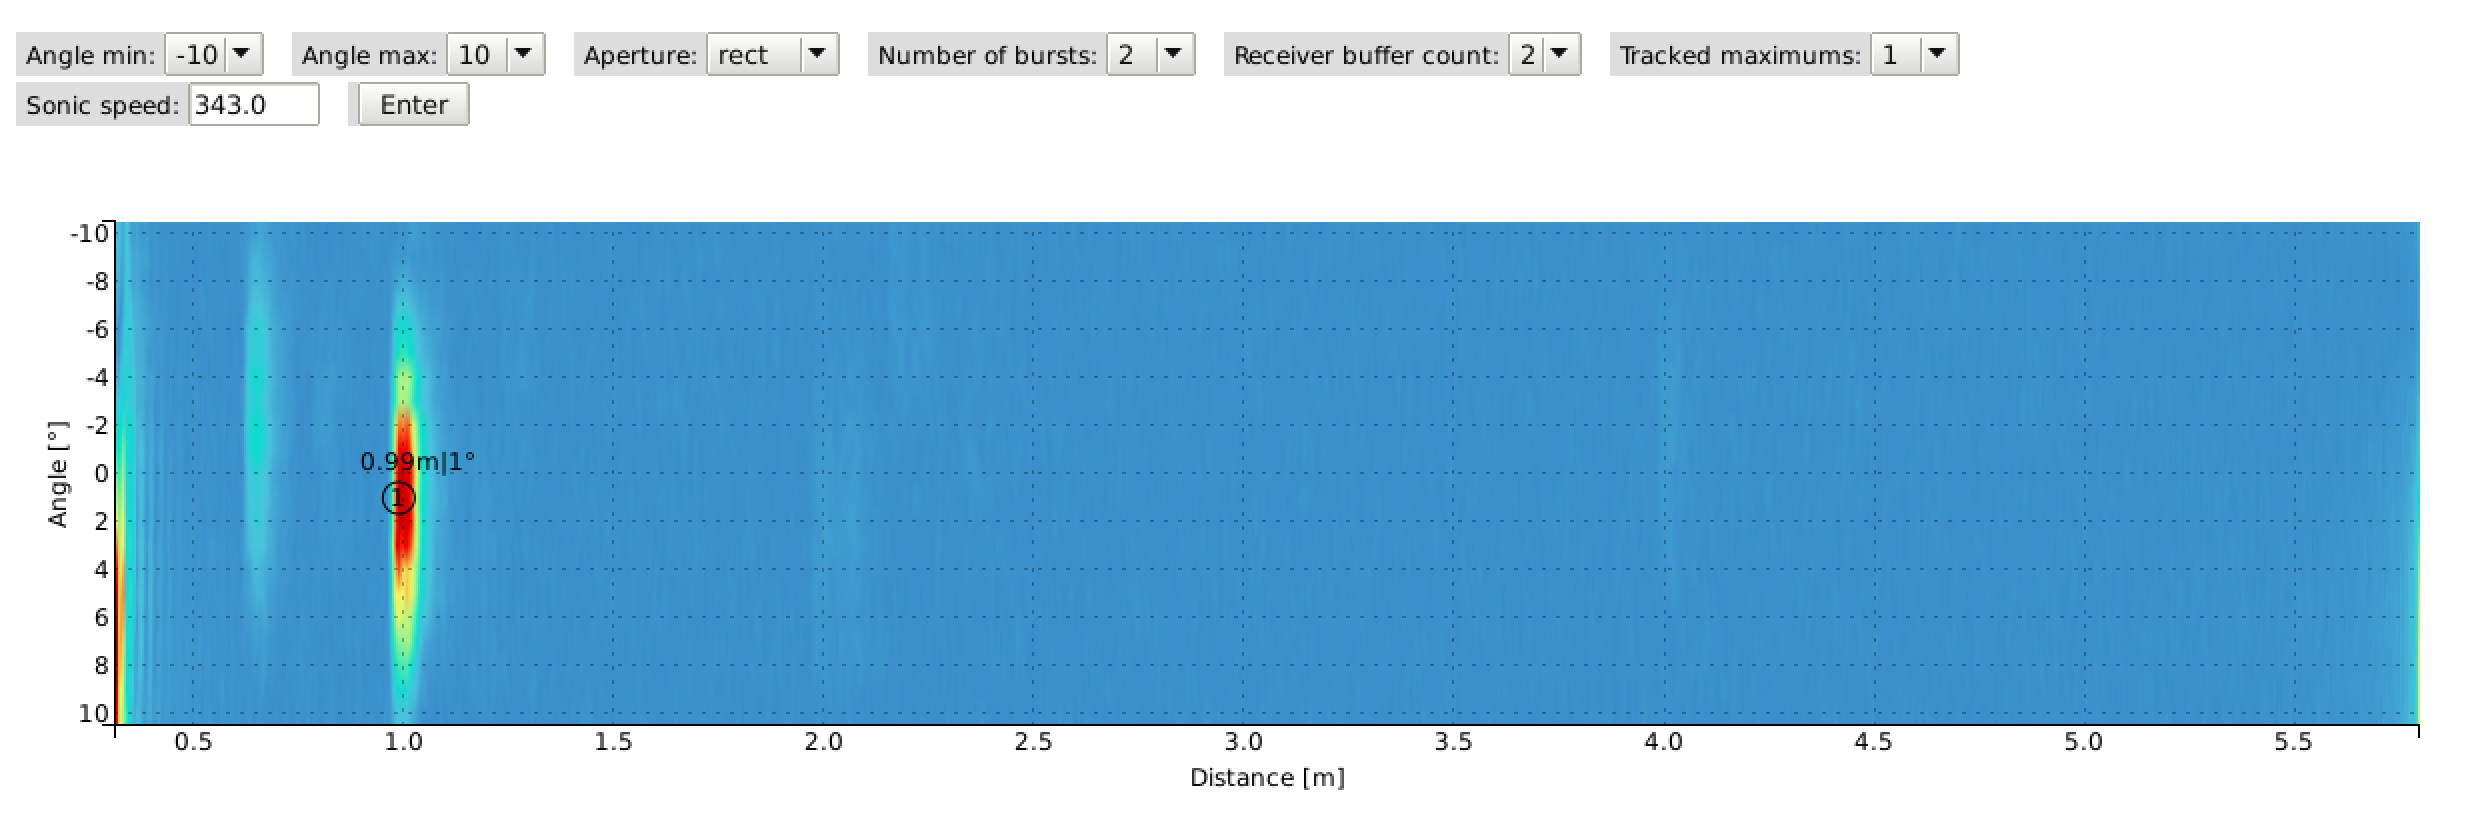
\includegraphics[width=\textwidth]{graphics/image_test_distance_01m.png}
\caption{1m: Maximum bei $0.99 \mathrm{m}$ und $1^{\circ}$} % picture caption
\label{fig:image_test_distance_01m}
%\end{figure}
%
%(Abb. \ref{fig:image1})
%%%%%%%%%%%%%%%%%%%%%%%%%%%%%%%%%%%%%%%%%%%%%%%%%%%%%%%%%%%%%%%%%%%%%%%%%%%%%%%%
\end{minipage}
\begin{minipage}{1.0\textwidth}
%%%%%%%%%%%%%%%%%%%%%%%%%%%%%%%%%%%%%%%%%%%%%%%%%%%%%%%%%%%%%%%%%%%%%%%%%%%%%%%%
% pictures
%\begin{figure}[htb]
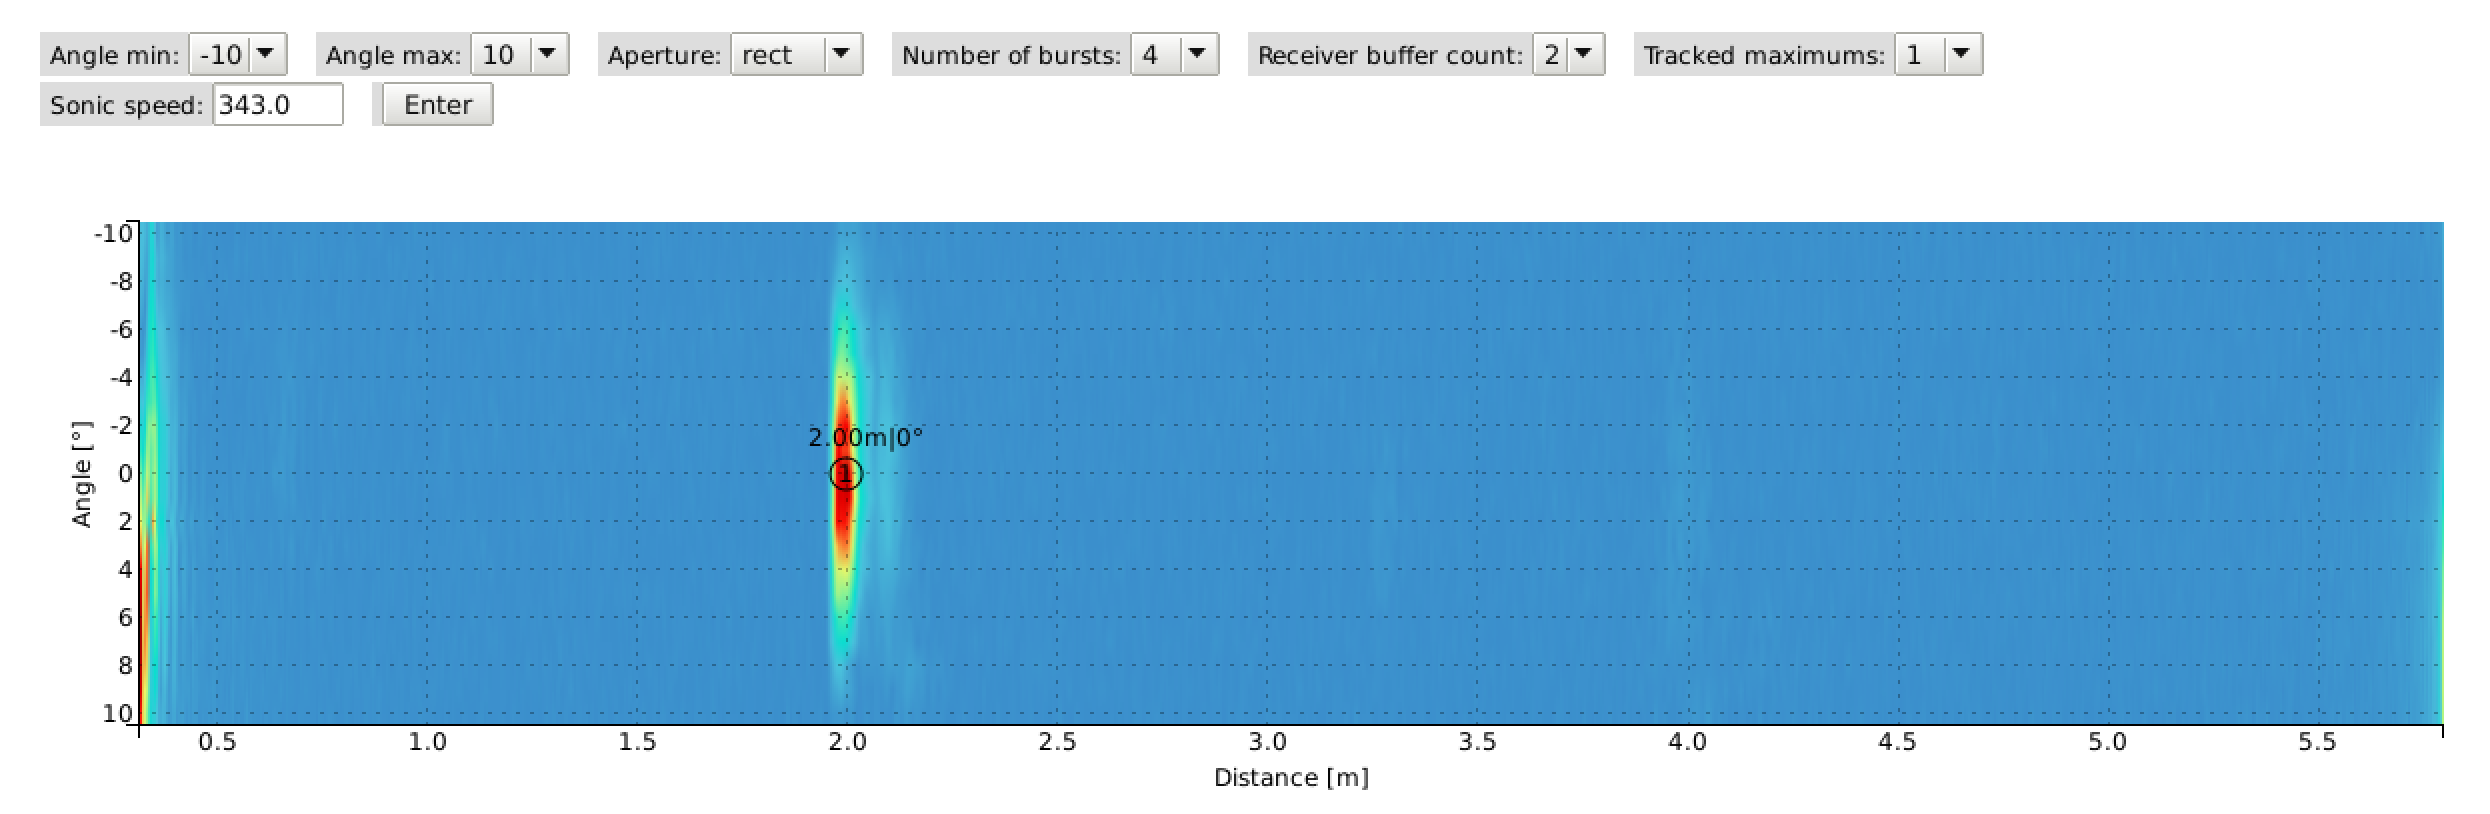
\includegraphics[width=\textwidth]{graphics/image_test_distance_02m.png}
\caption{2m: Maximum bei $2.00 \mathrm{m}$ und $0^{\circ}$} % picture caption
\label{fig:image_test_distance_02m}
%\end{figure}
%
%(Abb. \ref{fig:image1})
%%%%%%%%%%%%%%%%%%%%%%%%%%%%%%%%%%%%%%%%%%%%%%%%%%%%%%%%%%%%%%%%%%%%%%%%%%%%%%%%
\end{minipage}
\end{figure}
Für eine Distanz von $1.00 \mathrm{m}$ wird die Messung mit zwei Sendepulsen durchgeführt. Die Messabweichung zwischen dem gemessenem Referenzwert und dem im GUI abgelesenen Wert beträgt $-1 \mathrm{cm}$.

Bei einer Distanz von $2.00 \mathrm{m}$ wird die Messung mit vier Sendepulsen durchgeführt. Die Maximum-Tracking Funktion im GUI zeigt dabei genau $2.00 \mathrm{m}$ an.

\clearpage
\begin{figure}[htb]
\begin{minipage}{1.0\textwidth}
%%%%%%%%%%%%%%%%%%%%%%%%%%%%%%%%%%%%%%%%%%%%%%%%%%%%%%%%%%%%%%%%%%%%%%%%%%%%%%%%
% pictures
%\begin{figure}[htb]
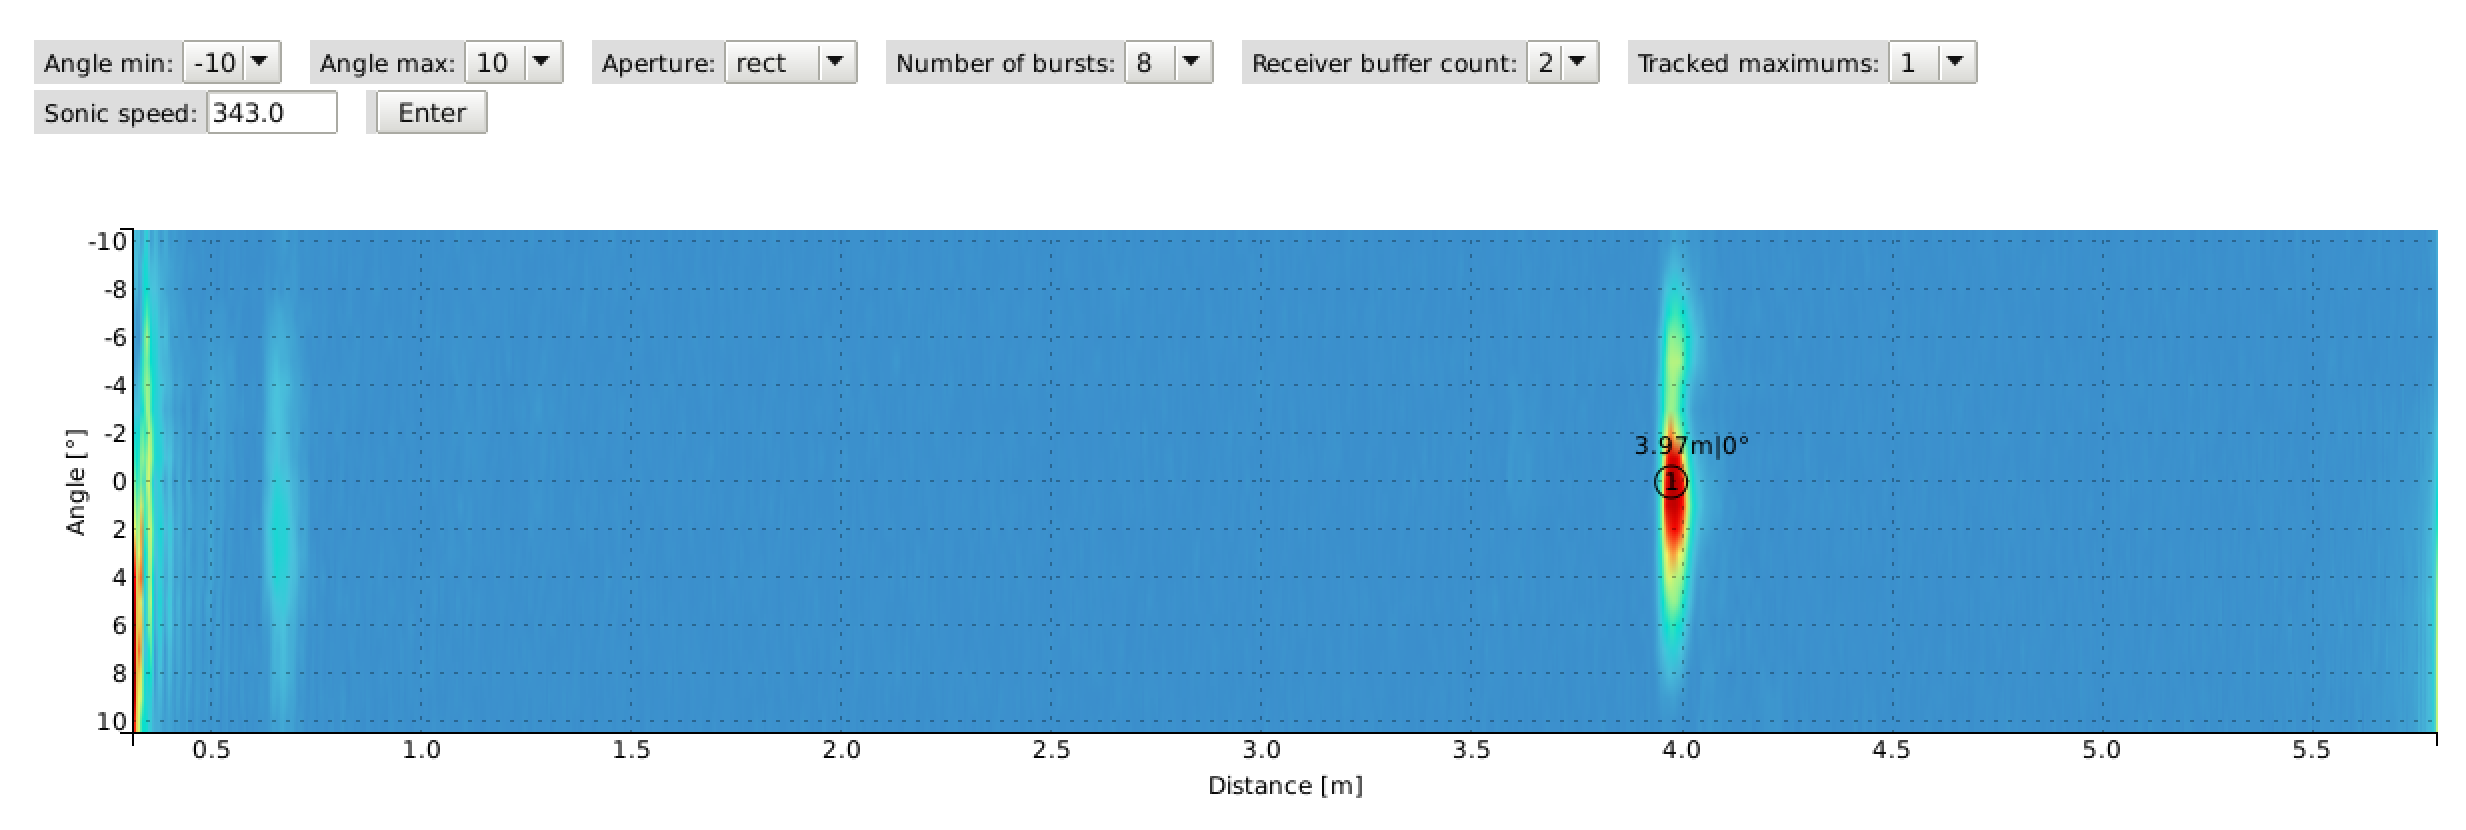
\includegraphics[width=\textwidth]{graphics/image_test_distance_04m.png}
\caption{4m: Maximum bei $3.97 \mathrm{m}$ und $0^{\circ}$} % picture caption
\label{fig:image_test_distance_04m}
%\end{figure}
%
%(Abb. \ref{fig:image1})
%%%%%%%%%%%%%%%%%%%%%%%%%%%%%%%%%%%%%%%%%%%%%%%%%%%%%%%%%%%%%%%%%%%%%%%%%%%%%%%%
\end{minipage}
\begin{minipage}{1.0\textwidth}
%%%%%%%%%%%%%%%%%%%%%%%%%%%%%%%%%%%%%%%%%%%%%%%%%%%%%%%%%%%%%%%%%%%%%%%%%%%%%%%%
% pictures
%\begin{figure}[htb]
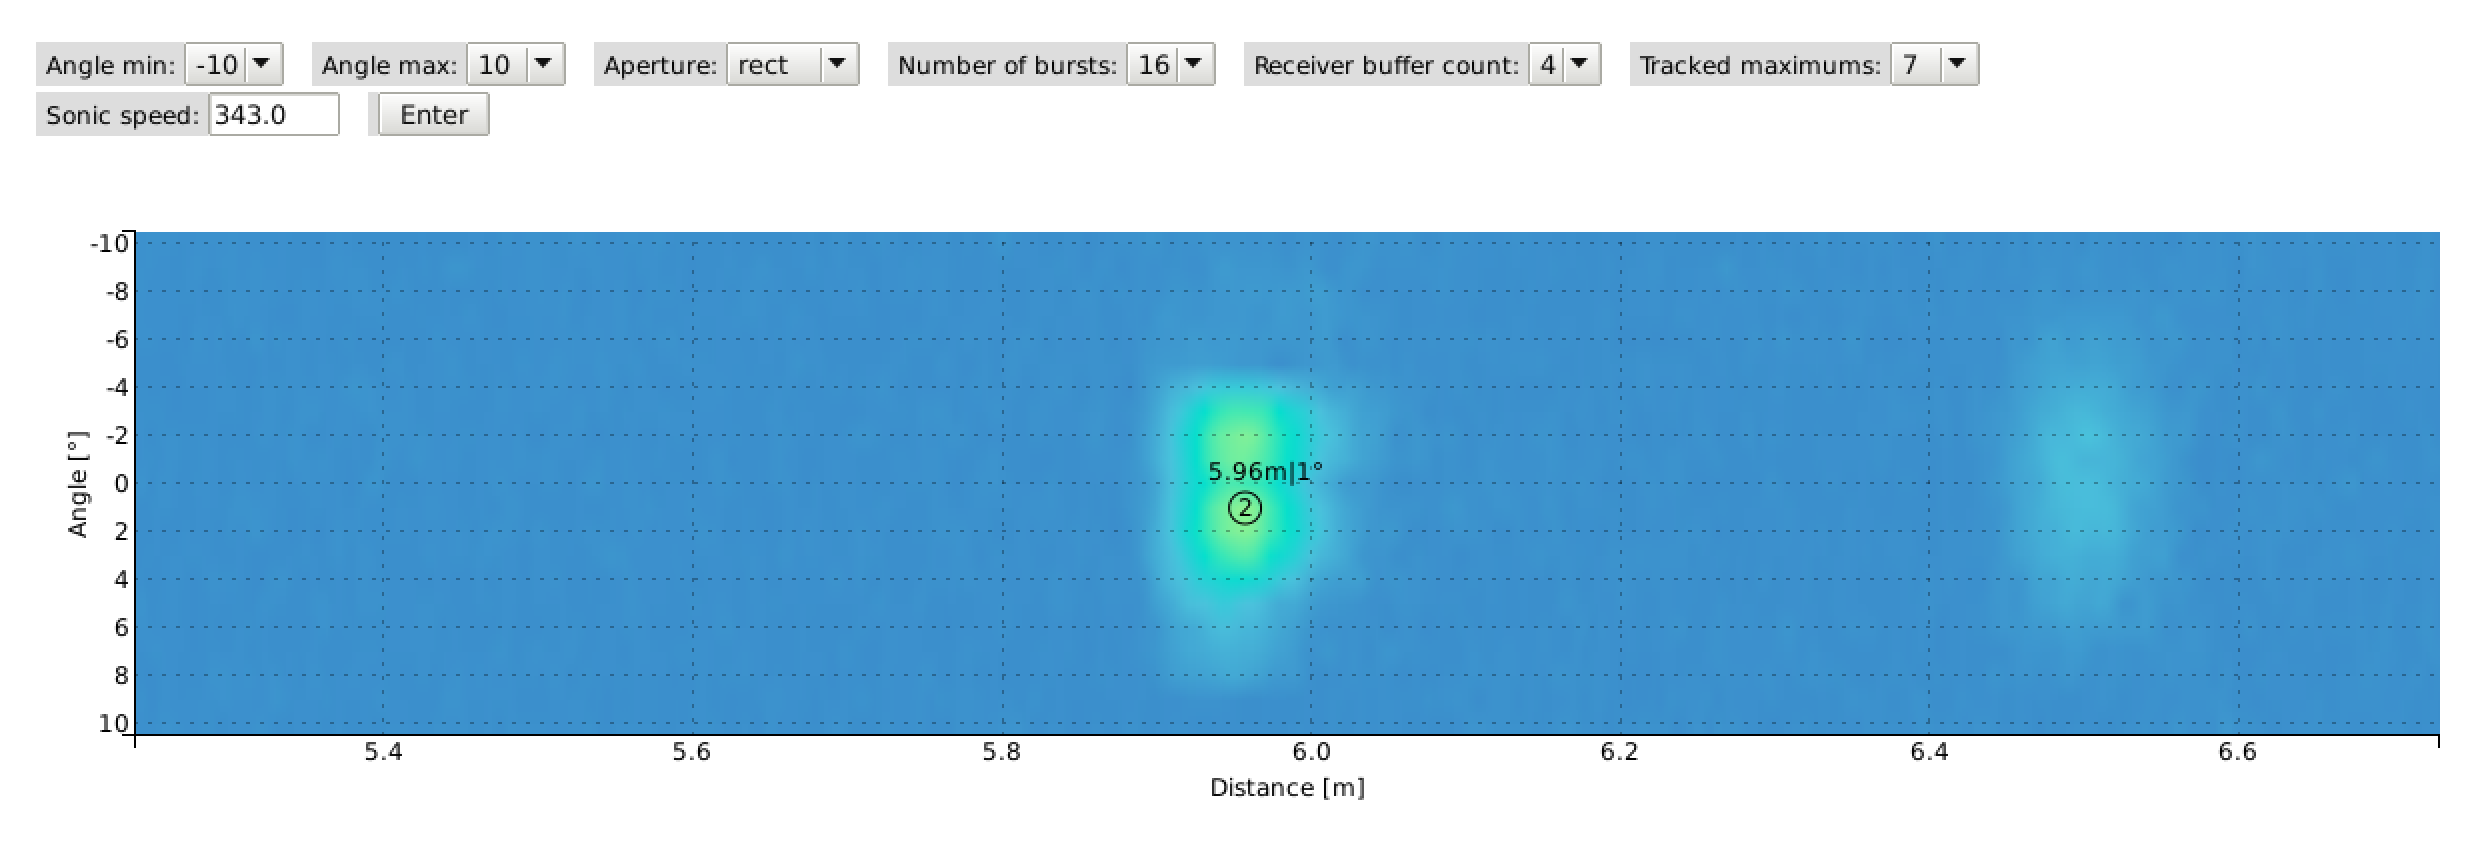
\includegraphics[width=\textwidth]{graphics/image_test_distance_06m.png}
\caption{6m: Maximum bei $5.96 \mathrm{m}$ und $1^{\circ}$} % picture caption
\label{fig:image_test_distance_06m}
%\end{figure}
%
%(Abb. \ref{fig:image1})
%%%%%%%%%%%%%%%%%%%%%%%%%%%%%%%%%%%%%%%%%%%%%%%%%%%%%%%%%%%%%%%%%%%%%%%%%%%%%%%%
\end{minipage}
\end{figure}

Bei der Messung für den Referenzwert von $4.00 \mathrm{m}$ wird die Anzahl Sendepulse auf acht erhöht. Die Messabweichung beträgt dabei $-3 \mathrm{cm}$.

Für eine Distanz von $6.00 \mathrm{m}$ ist trotz einer Erhöhung der Anzahl Sendepulse auf 16 ein Abfall in der gemessenen Amplitude des Echos festzustellen. Die Messabweichung zwischen dem von der Maximum-Tracking Funktion gefunden Wert und der Referenzmessung beträgt $-4 \mathrm{cm}$. Ein zweites, störendes Maximum ist in der Abbildung \ref{fig:image_test_distance_06m} bei einer Distanz von ungefähr $6.5 \mathrm{m}$ zu erkennen.
\clearpage
\begin{figure}[htb]
\begin{minipage}{1.0\textwidth}
%%%%%%%%%%%%%%%%%%%%%%%%%%%%%%%%%%%%%%%%%%%%%%%%%%%%%%%%%%%%%%%%%%%%%%%%%%%%%%%%
% pictures
%\begin{figure}[htb]
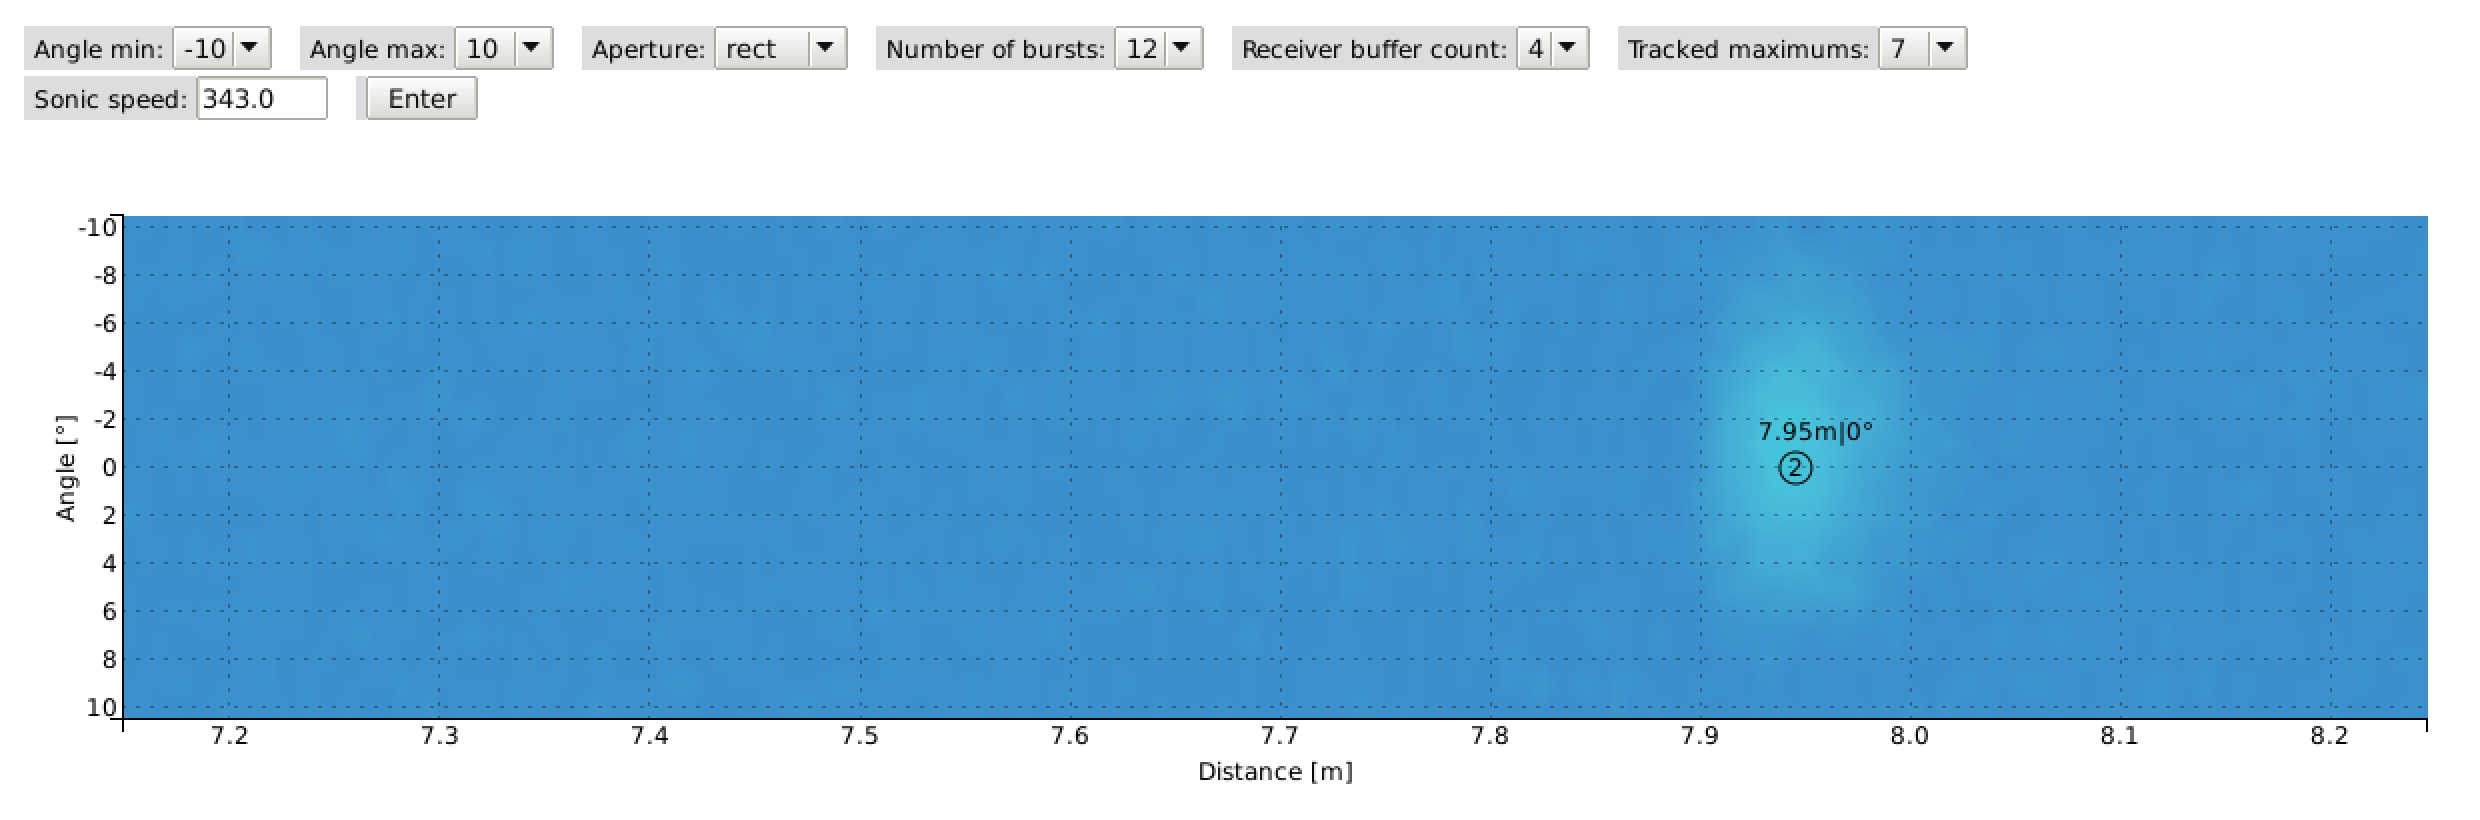
\includegraphics[width=\textwidth]{graphics/image_test_distance_08m.png}
\caption{8m: Maximum bei $7.95 \mathrm{m}$ und $0^{\circ}$} % picture caption
\label{fig:image_test_distance_08m}
%\end{figure}
%
%(Abb. \ref{fig:image1})
%%%%%%%%%%%%%%%%%%%%%%%%%%%%%%%%%%%%%%%%%%%%%%%%%%%%%%%%%%%%%%%%%%%%%%%%%%%%%%%%
\end{minipage}
\begin{minipage}{1.0\textwidth}
%%%%%%%%%%%%%%%%%%%%%%%%%%%%%%%%%%%%%%%%%%%%%%%%%%%%%%%%%%%%%%%%%%%%%%%%%%%%%%%%
% pictures
%\begin{figure}[htb]
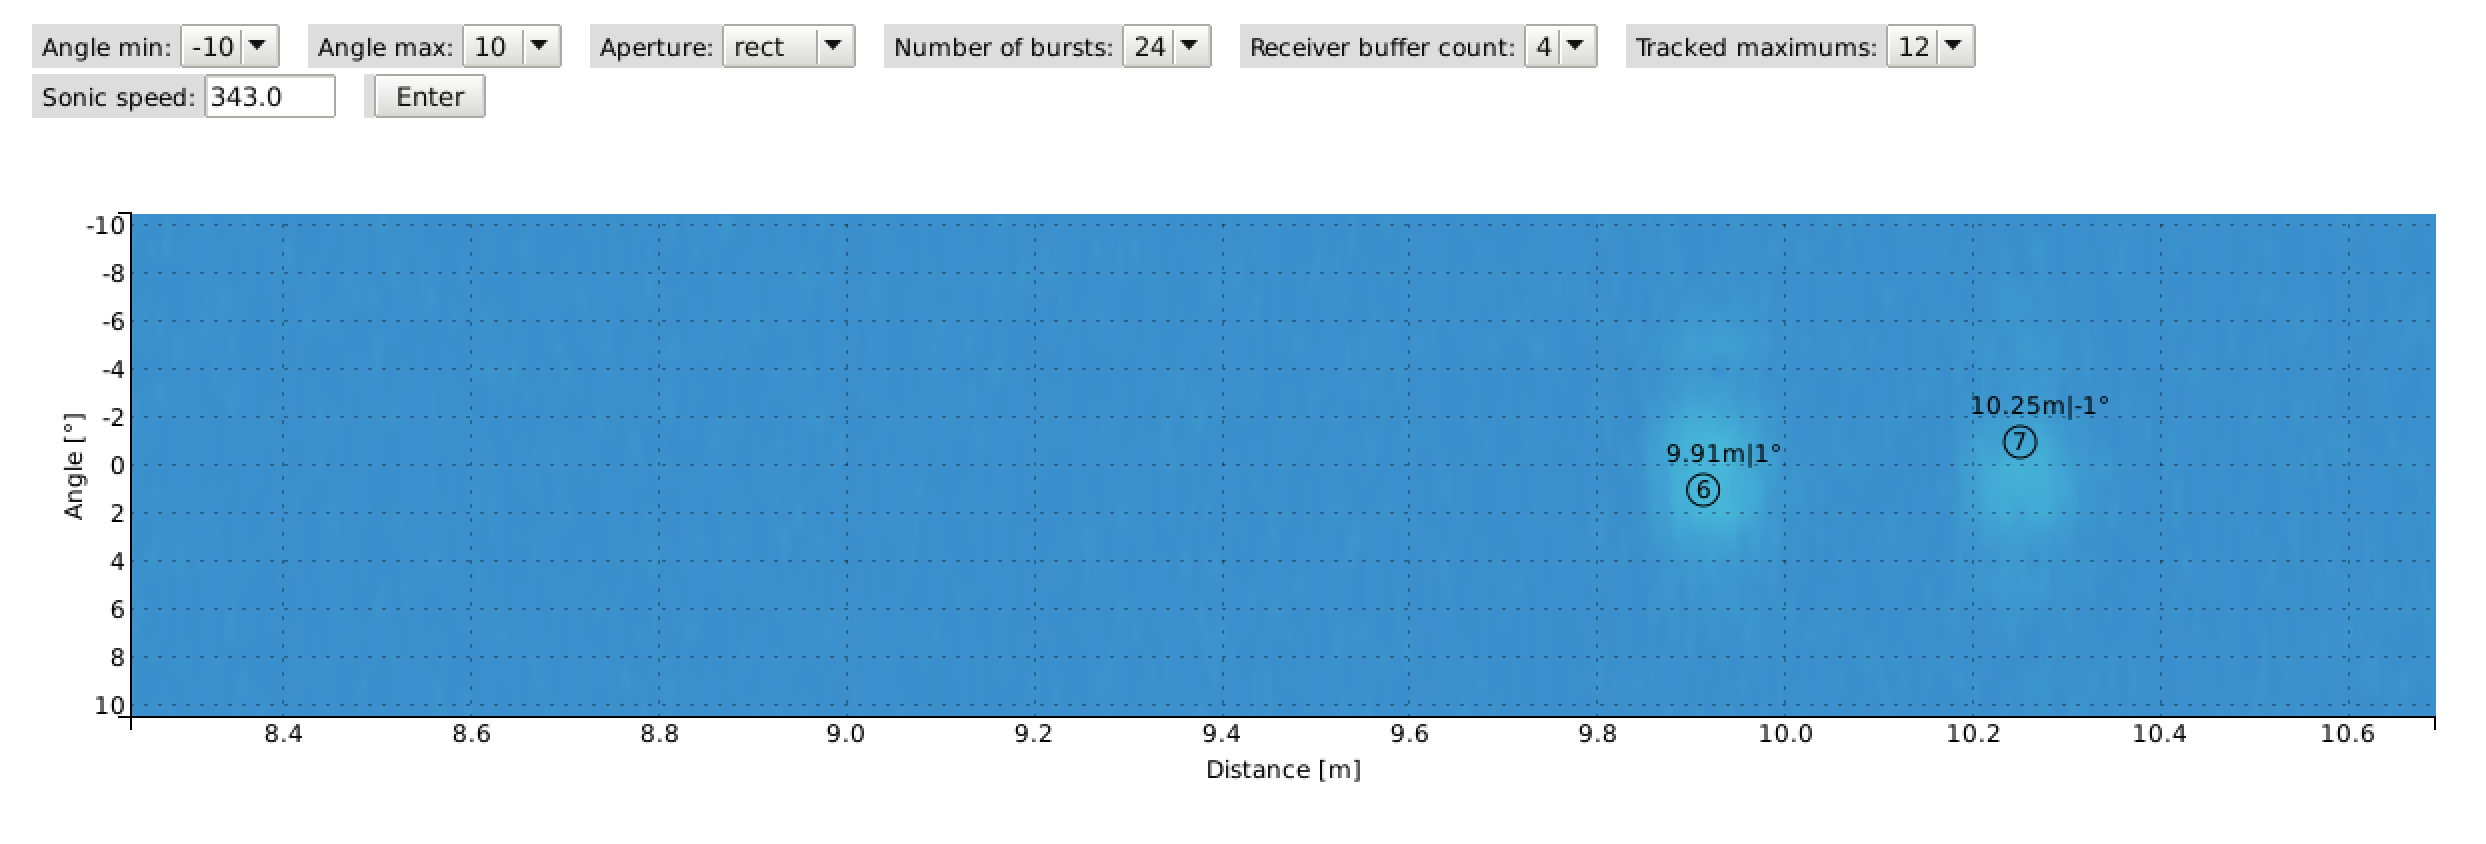
\includegraphics[width=\textwidth]{graphics/image_test_distance_10m.png}
\caption{10m: Maxima bei $9.91 \mathrm{m}$ und $1^{\circ}$ und bei $10.25 \mathrm{m}$ und $-1^{\circ}$} % picture caption
\label{fig:image_test_distance_10m}
%\end{figure}
%
%(Abb. \ref{fig:image1})
%%%%%%%%%%%%%%%%%%%%%%%%%%%%%%%%%%%%%%%%%%%%%%%%%%%%%%%%%%%%%%%%%%%%%%%%%%%%%%%%
\end{minipage}
\end{figure}

Für grosse Distanzen werden vermehrt störende Echos von anderen Objekten im Raum empfangen. Die Amplitude des zu messenden Echos wird bei einer Distanz $8.00 \mathrm{m}$ von der Maximum-Tracking Funktion nur noch als zweitgrösster Peak erkannt. Die Messabweichung beträgt dabei $-5 \mathrm{cm}$. Es ist zu erwähnen, dass das Ultraschall Phased Array für derart grosse Distanzen genau auf die Wand ausgerichtet sein muss, ansonsten ist das von der Wand reflektierte Echo zu schwach.

Ab einer Distanz von $8 \mathrm{m}$ wird die Distanzmessung problematisch. So sind im Bereich von $\pm 30 \mathrm{cm}$ um die gemessene Referenzdistanz von {$10.00 \mathrm{m}$} zwei Maxima vorhanden und es ist nicht klar welches von der Wand stammt.

\clearpage
\begin{figure}[htb]
\begin{minipage}{1.0\textwidth}
%%%%%%%%%%%%%%%%%%%%%%%%%%%%%%%%%%%%%%%%%%%%%%%%%%%%%%%%%%%%%%%%%%%%%%%%%%%%%%%%
% pictures
%\begin{figure}[htb]
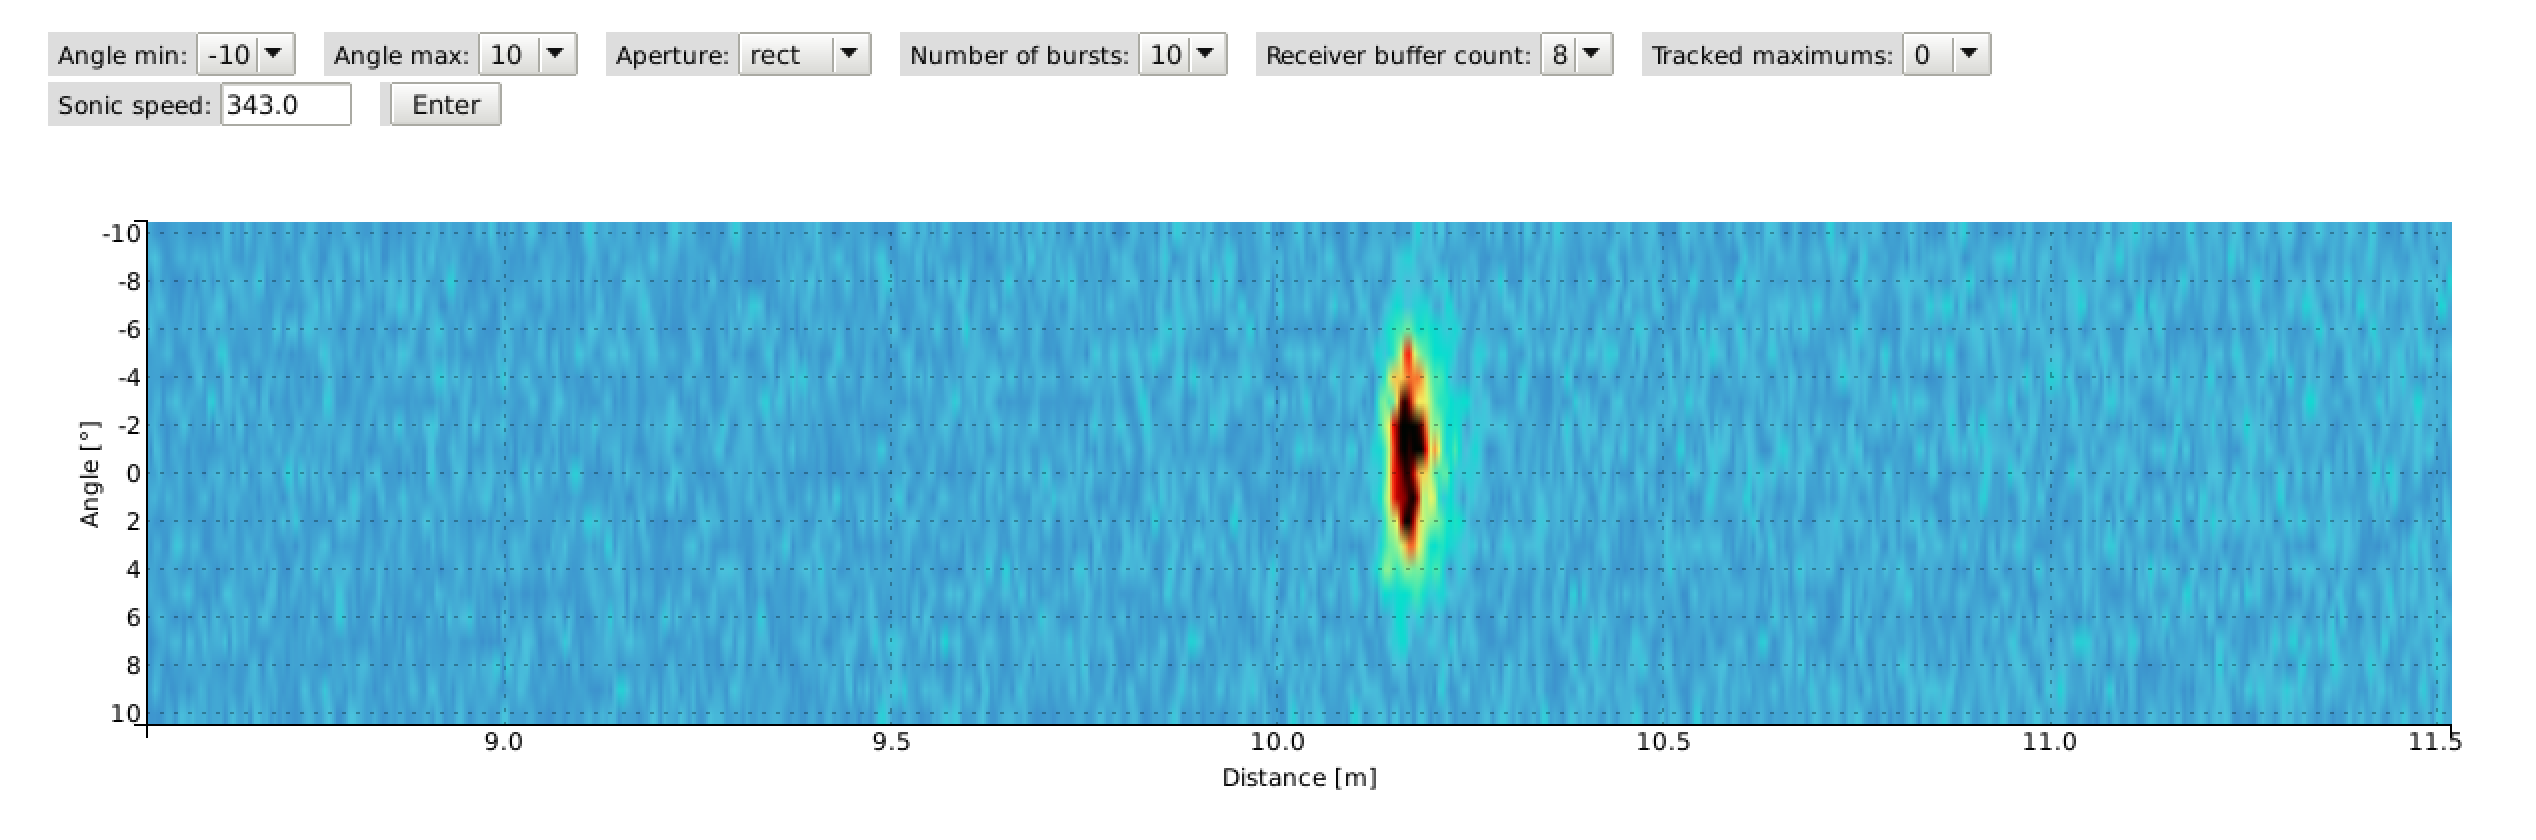
\includegraphics[width=\textwidth]{graphics/image_test_distance_10m_scaled.png}
\caption{Messung für $10 \mathrm{m}$ mit skalierten Werten} % picture caption
\label{fig:image_test_distance_10m_scaled}
%\end{figure}
%
%(Abb. \ref{fig:image1})
%%%%%%%%%%%%%%%%%%%%%%%%%%%%%%%%%%%%%%%%%%%%%%%%%%%%%%%%%%%%%%%%%%%%%%%%%%%%%%%%
\end{minipage}
\begin{minipage}{1.0\textwidth}
%%%%%%%%%%%%%%%%%%%%%%%%%%%%%%%%%%%%%%%%%%%%%%%%%%%%%%%%%%%%%%%%%%%%%%%%%%%%%%%%
% pictures
%\begin{figure}[htb]
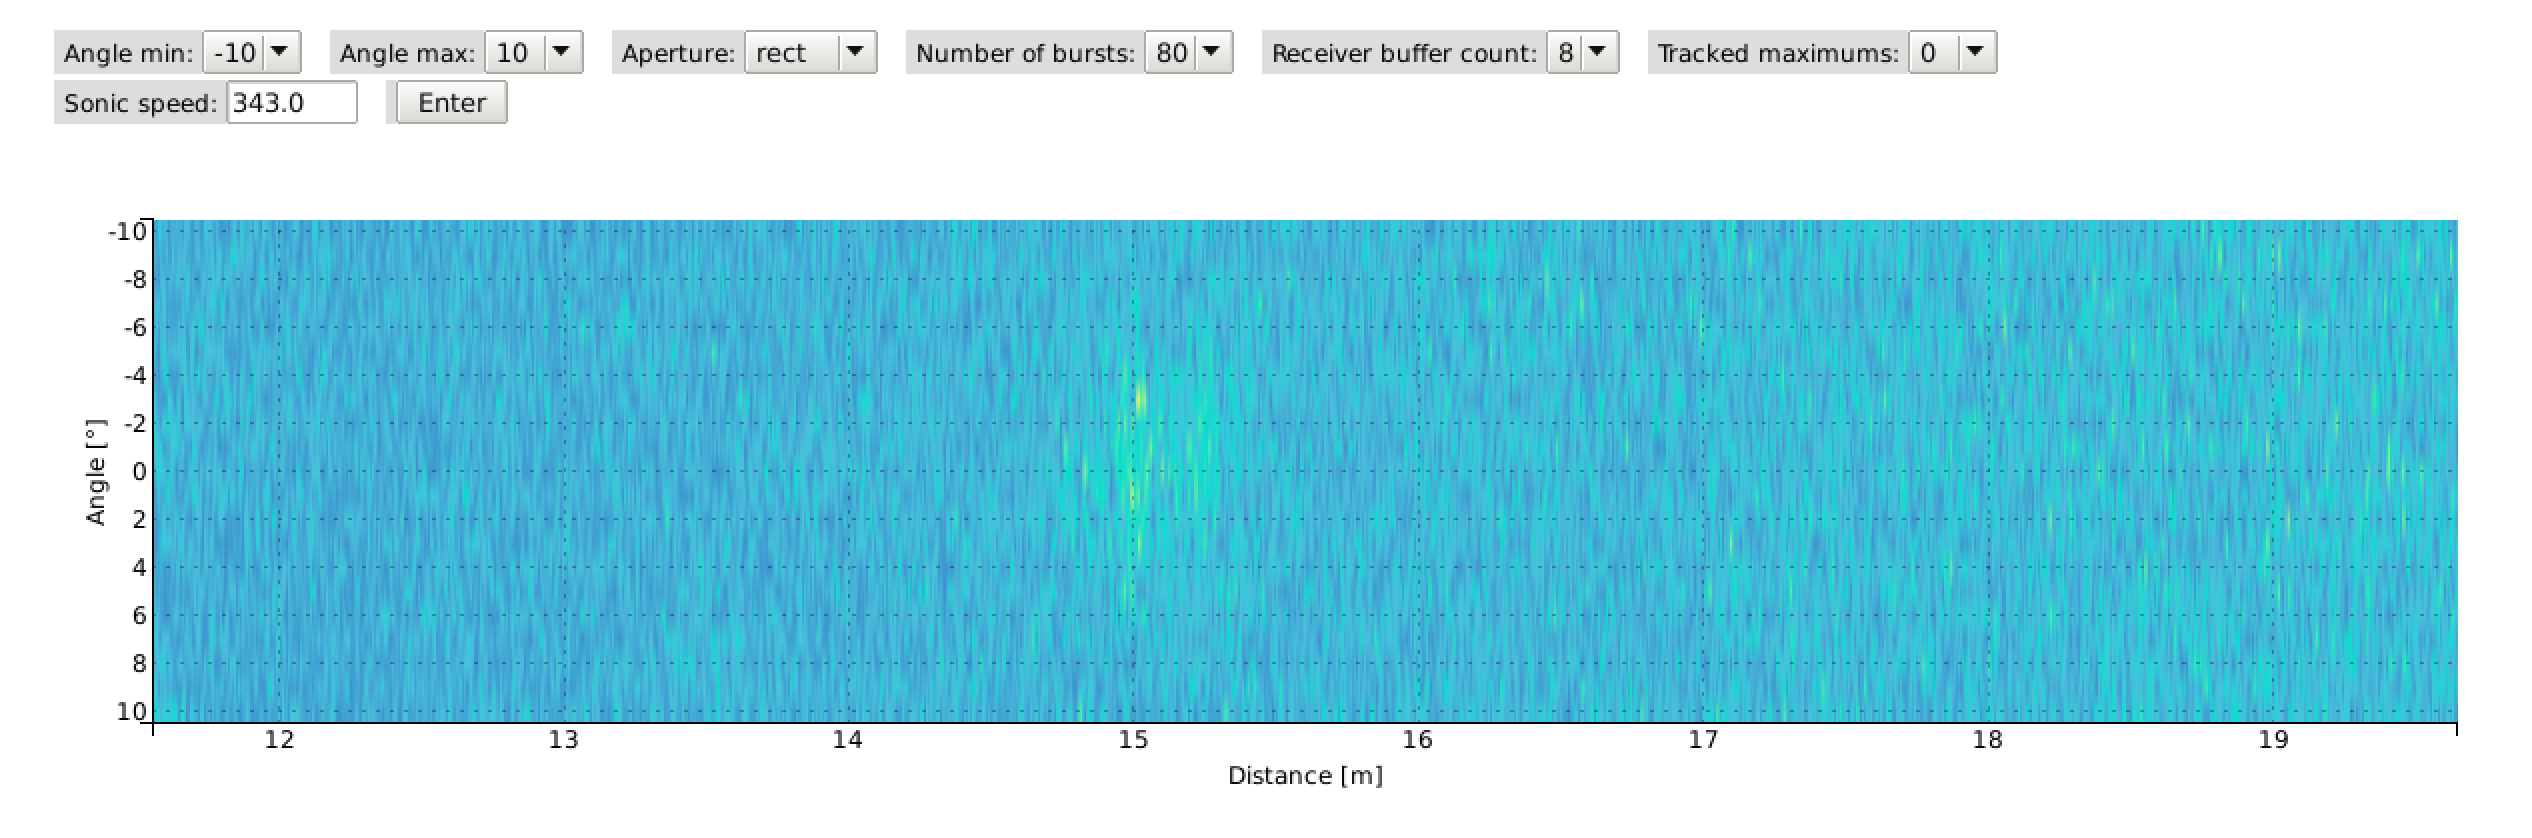
\includegraphics[width=\textwidth]{graphics/image_test_distance_15m_scaled.png}
\caption{Messung für $15 \mathrm{m}$ mit skalierten Werten} % picture caption
\label{fig:image_test_distance_15m_scaled}
%\end{figure}
%
%(Abb. \ref{fig:image1})
%%%%%%%%%%%%%%%%%%%%%%%%%%%%%%%%%%%%%%%%%%%%%%%%%%%%%%%%%%%%%%%%%%%%%%%%%%%%%%%%
\end{minipage}
\end{figure}
Werden die Werte des dargestellten Signals linear mit der Distanz skaliert, so werden Werte stärker erhöht, die aufgrund der Dämpfung abgeschwächt sind. Dies ist zwar mathematisch nicht korrekt und nur ein erster Versuch zur Weiterentwicklung des Projektes (siehe Weiterentwicklung im Kapitel \ref{sec:schlusswort}), der positive Effekt auf die Sichtbarkeit von weit entfernten Objekten soll hier aber trotzdem kurz aufgezeigt werden. Dieses skalierte Signal ist in Abbildung \ref{fig:image_test_distance_10m_scaled} dargestellt.

Aufgrund des mit der Skalierung angehobenen Rauschpegels geht das Echo ab einer Distanz von $15 \mathrm{m}$ fast im Rauschen unter. Dies ist in Abbildung \ref{fig:image_test_distance_15m_scaled} zu sehen.

\clearpage
%%%%%%%%%%%%%%%%%%%%%%%%%%%%%%%%%%%%%%%%%%%%%%%%%%%%%%%%%%%%%%%%%%%%%%%%%%%%%%%%
%%%%%%%%%%%%%%%%%%%%%%%%%%%%%%%%%%%%%%%%%%%%%%%%%%%%%%%%%%%%%%%%%%%%%%%%%%%%%%%%
%%%%%%%%%%%%%%%%%%%%%%%%%%%%%%%%%%%%%%%%%%%%%%%%%%%%%%%%%%%%%%%%%%%%%%%%%%%%%%%%
\subsection{Objekterkennung anhand ausgewählter Beispiele}\label{sec:objekterkennung_anhand_ausgewählter_beispiele}
Im Folgenden sind ausgewählte Beispiele von Umgebungsscans aufgeführt und kommentiert. Weitere Bilder von Umgebungsscans sind im Anhang \ref{sec:appendix_objekterkennung} zu finden.

Das zur Dämpfung unerwünschter Reflexionen verwendete Schaumstoffstück (für die Messungen im Kapitel \ref{sec:messung_der_empfangsseitigen_richtcharakteristik} und \ref{sec:distanzmessungen})  wird als Testobjekt im reflexionsarmen Halbraum vermessen. Das Schaumstoffstück ist $40 \mathrm{cm}$ breit und wird in einer Entfernung von $1.5 \mathrm{m}$ vor dem Array aufgestellt. Bei einen Winkel von $20^{\circ}$ und frontaler Ausrichtung auf das Array entsteht mit $20$ Sendepulsen die Abbildung \ref{fig:image_test_obj_schaumstoff_20deg_0}. Der vom Schaumstoffstück eingenommene Winkel von ca. $15^{\circ}$ ist auf dem Bild erstaunlich gut erkennbar.
Die Mehrfachechos in der Nähe des Arrays stammen von einem Metallhebel am Stativ.

Wird das Schaumstoffstück in einem Winkel von $0^{\circ}$ frontal vor dem Array aufgestellt, entsteht das Bild \ref{fig:image_test_obj_schaumstoff_0deg}. Der Sprung um $0^{\circ}$ ist auf die minimale Verzögerung beim Einschalten der PWM-Kanäle zurückzuführen (ebenfalls zu sehen in Abbildung \ref{fig:plot_test_characteristic_rect_0_polar}).

Für die Abbildung \ref{fig:image_test_obj_person_0} hat sich eine Person im reflexionsarmen Halbraum vor das Array gestellt und für die Abbildung \ref{fig:image_test_obj_person_1} sind es zwei Personen im Freien.

Die Messung mit dem Schaumstoffstück in einem Winkel von $20^{\circ}$ (Abbildung \ref{fig:image_test_obj_schaumstoff_20deg_0}) wird wiederholt, jedoch wird dieses nicht dem Array zugewandt, sondern parallel zum Array aufgestellt. Dadurch ensteht die Abbildung \ref{fig:image_test_obj_schaumstoff_20deg_1}. Es ist eine Problematik bei der Objekterkennung mittels gerichtetem Schallkegel zu sehen. Schall von Objekten, welche nicht dem Array zugewandt sind, wird nicht zwingend in die Richtung des Arrays zurückgeworfen (siehe Kapitel \ref{sec:reflexion_und_transmission_von_schall_beim_auftreffen_auf_grenzflaechen}).

Zum Abschluss ist ein Bild mit einem Mikrophonstativ als Test-Objekt zu sehen. Es handelt sich dabei um eine Metallstange mit ca. $3 \mathrm{cm}$ Durchmesser im Abstand von $2.00 \mathrm{m}$ und in einem Winkel von $20^{\circ}$. Die Messung wird mit 20 Sendepulsen durchgeführt. Dabei entsteht die Abbildung \ref{fig:image_test_obj_mikrophonstaender}. Im Hintergrund ist die offene Türe zum reflexionsarmen Halbraum erkennbar.

\clearpage
\begin{figure}[htb]
\begin{minipage}{1.0\textwidth}
%%%%%%%%%%%%%%%%%%%%%%%%%%%%%%%%%%%%%%%%%%%%%%%%%%%%%%%%%%%%%%%%%%%%%%%%%%%%%%%%
% pictures
%\begin{figure}[htb]
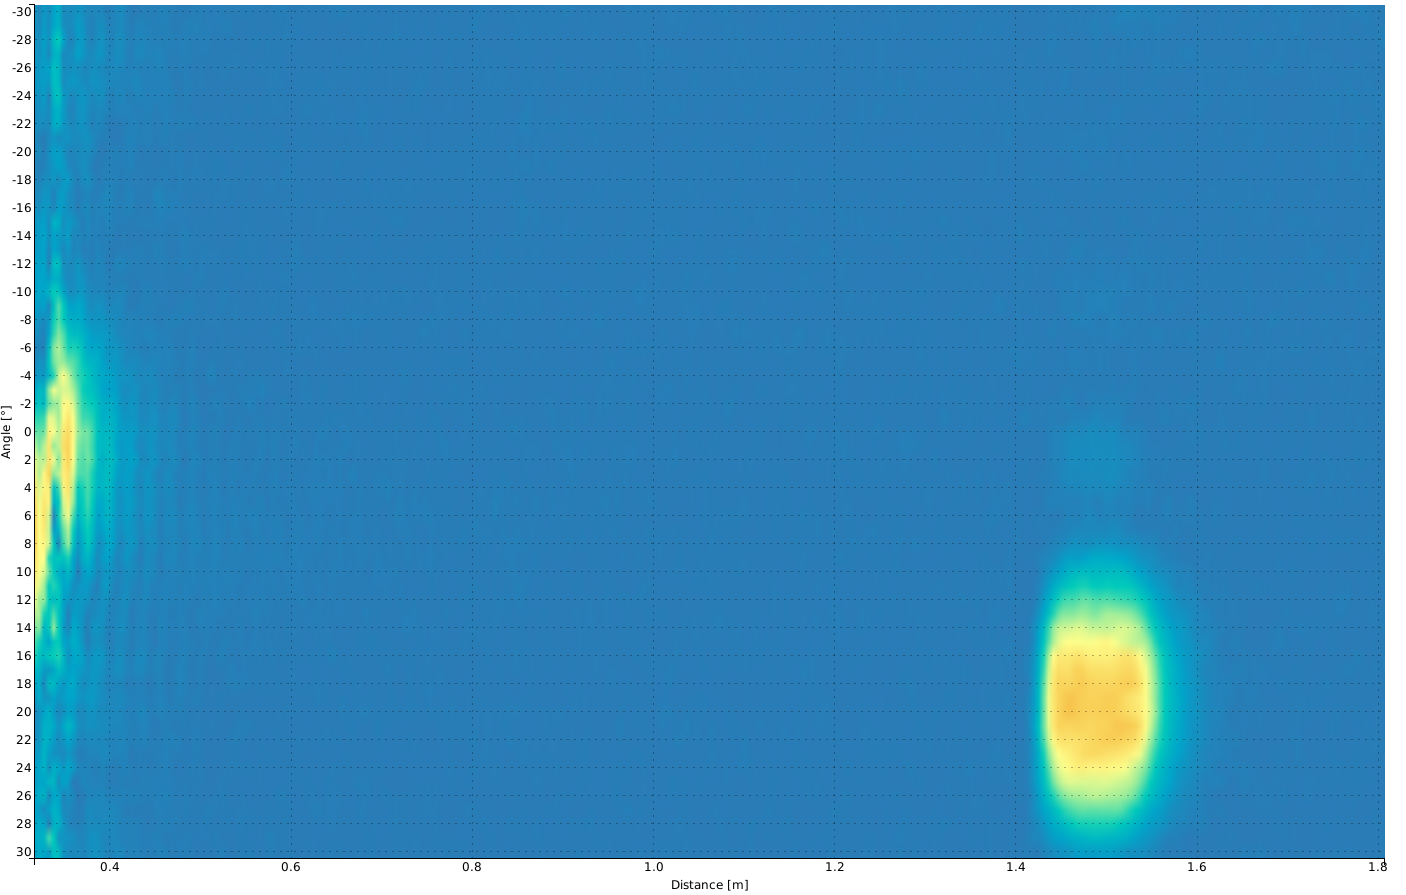
\includegraphics[width=\textwidth]{graphics/image_test_obj_schaumstoff_20deg_0.png}
\caption{Schaumstoffstück bei $1.5 \mathrm{m}$ und $20^{\circ}$, 20 Sendepulse} % picture caption
\label{fig:image_test_obj_schaumstoff_20deg_0}
%\end{figure}
%
%(Abb. \ref{fig:image1})
%%%%%%%%%%%%%%%%%%%%%%%%%%%%%%%%%%%%%%%%%%%%%%%%%%%%%%%%%%%%%%%%%%%%%%%%%%%%%%%%
\end{minipage}
\begin{minipage}{1.0\textwidth}
%%%%%%%%%%%%%%%%%%%%%%%%%%%%%%%%%%%%%%%%%%%%%%%%%%%%%%%%%%%%%%%%%%%%%%%%%%%%%%%%
% pictures
%\begin{figure}[htb]
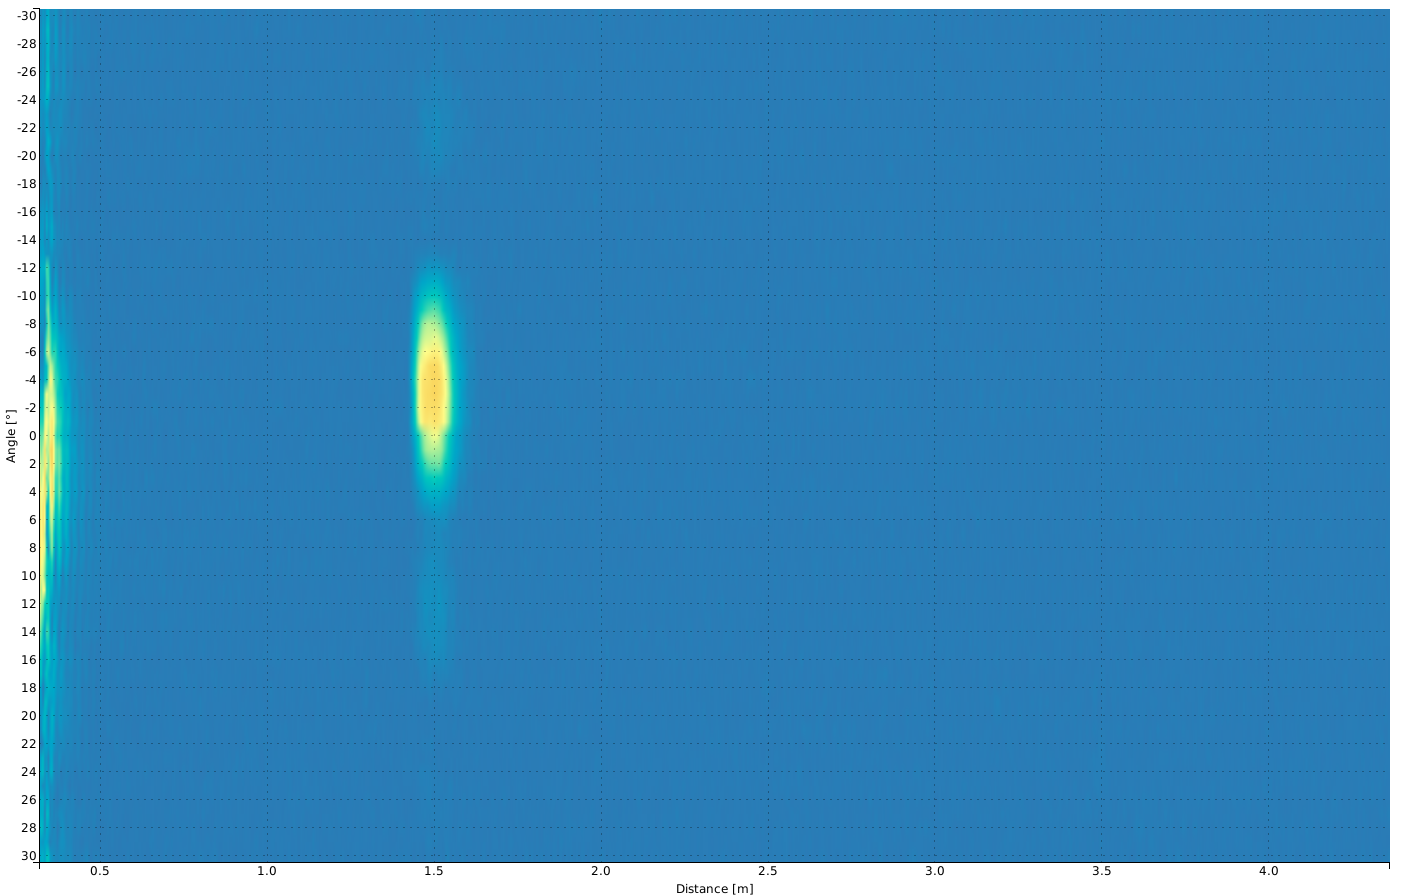
\includegraphics[width=\textwidth]{graphics/image_test_obj_schaumstoff_0deg.png}
\caption{Schaumstoffstück bei $1.5 \mathrm{m}$ und $0^{\circ}$, 20 Sendepulse} % picture caption
\label{fig:image_test_obj_schaumstoff_0deg}
%\end{figure}
%
%(Abb. \ref{fig:image1})
%%%%%%%%%%%%%%%%%%%%%%%%%%%%%%%%%%%%%%%%%%%%%%%%%%%%%%%%%%%%%%%%%%%%%%%%%%%%%%%%
\end{minipage}
\end{figure}


\clearpage
\begin{figure}[htb]
\begin{minipage}{1.0\textwidth}
%%%%%%%%%%%%%%%%%%%%%%%%%%%%%%%%%%%%%%%%%%%%%%%%%%%%%%%%%%%%%%%%%%%%%%%%%%%%%%%%
% pictures
%\begin{figure}[htb]
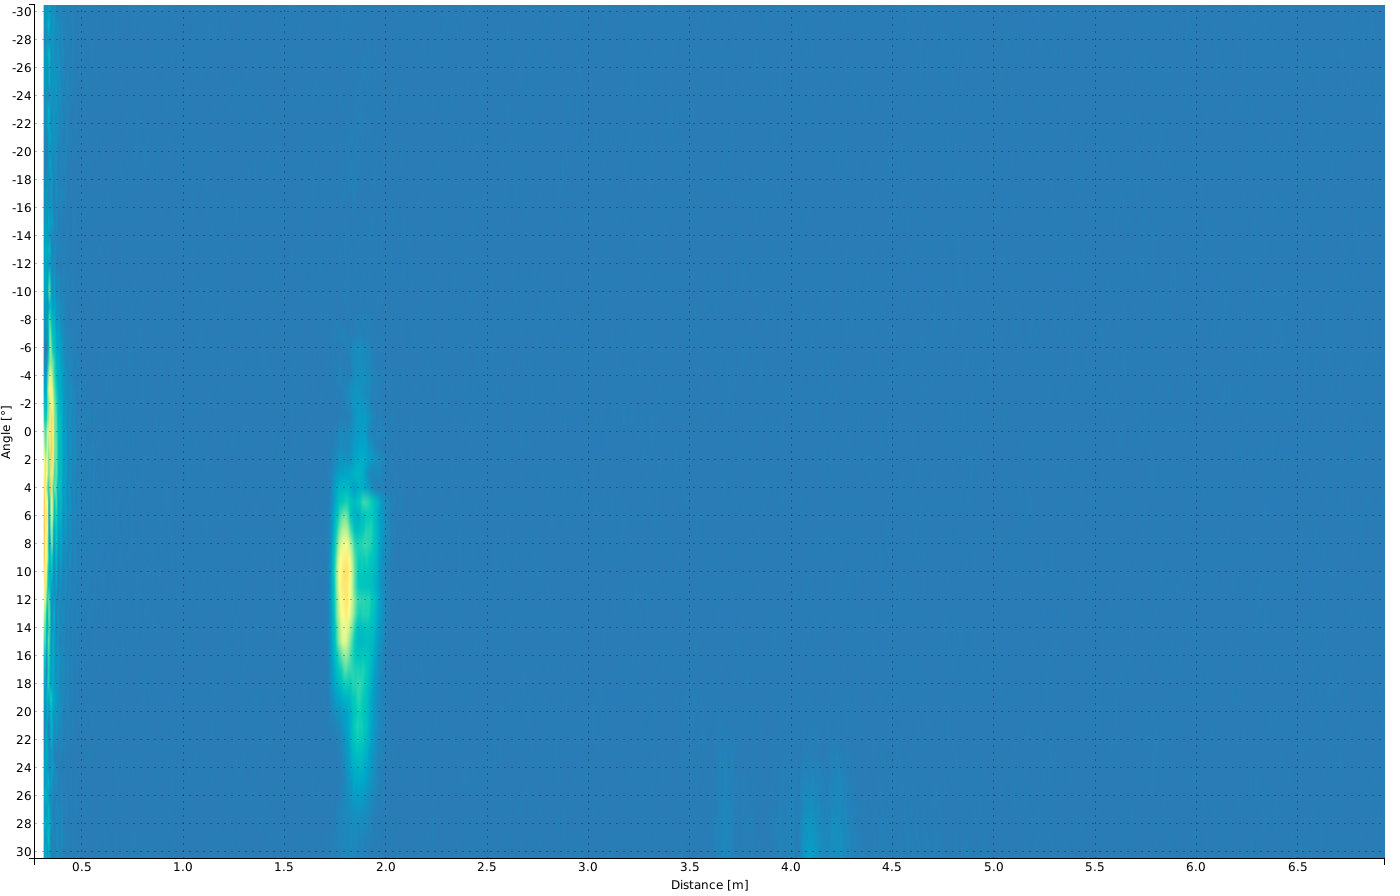
\includegraphics[width=\textwidth]{graphics/image_test_obj_person_0.png}
\caption{Person im reflexionsarmen Halbraum} % picture caption
\label{fig:image_test_obj_person_0}
%\end{figure}
%
%(Abb. \ref{fig:image1})
%%%%%%%%%%%%%%%%%%%%%%%%%%%%%%%%%%%%%%%%%%%%%%%%%%%%%%%%%%%%%%%%%%%%%%%%%%%%%%%%
\end{minipage}
\begin{minipage}{1.0\textwidth}
%%%%%%%%%%%%%%%%%%%%%%%%%%%%%%%%%%%%%%%%%%%%%%%%%%%%%%%%%%%%%%%%%%%%%%%%%%%%%%%%
% pictures
%\begin{figure}[htb]
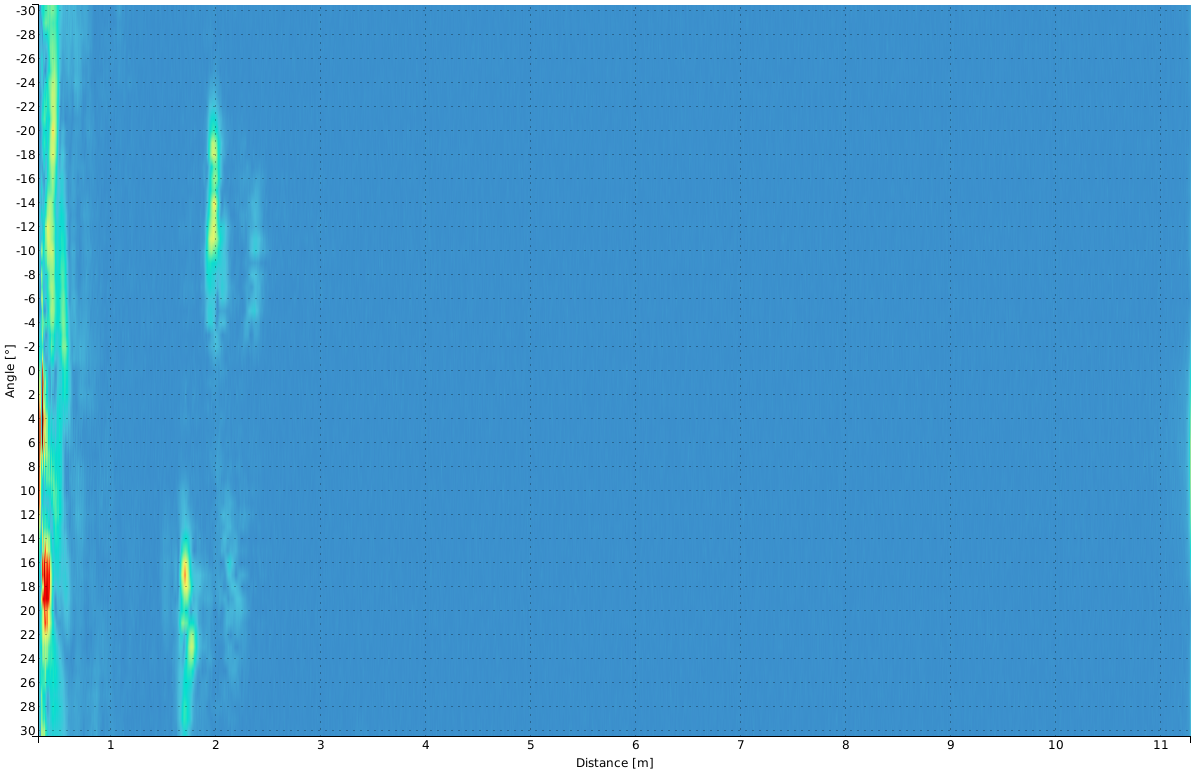
\includegraphics[width=\textwidth]{graphics/image_test_obj_person_1.png}
\caption{2 Personen im Freien} % picture caption
\label{fig:image_test_obj_person_1}
%\end{figure}
%
%(Abb. \ref{fig:image1})
%%%%%%%%%%%%%%%%%%%%%%%%%%%%%%%%%%%%%%%%%%%%%%%%%%%%%%%%%%%%%%%%%%%%%%%%%%%%%%%%
\end{minipage}
\end{figure}


\clearpage
\begin{figure}[htb]
\begin{minipage}{1.0\textwidth}
%%%%%%%%%%%%%%%%%%%%%%%%%%%%%%%%%%%%%%%%%%%%%%%%%%%%%%%%%%%%%%%%%%%%%%%%%%%%%%%%
% pictures
%\begin{figure}[htb]
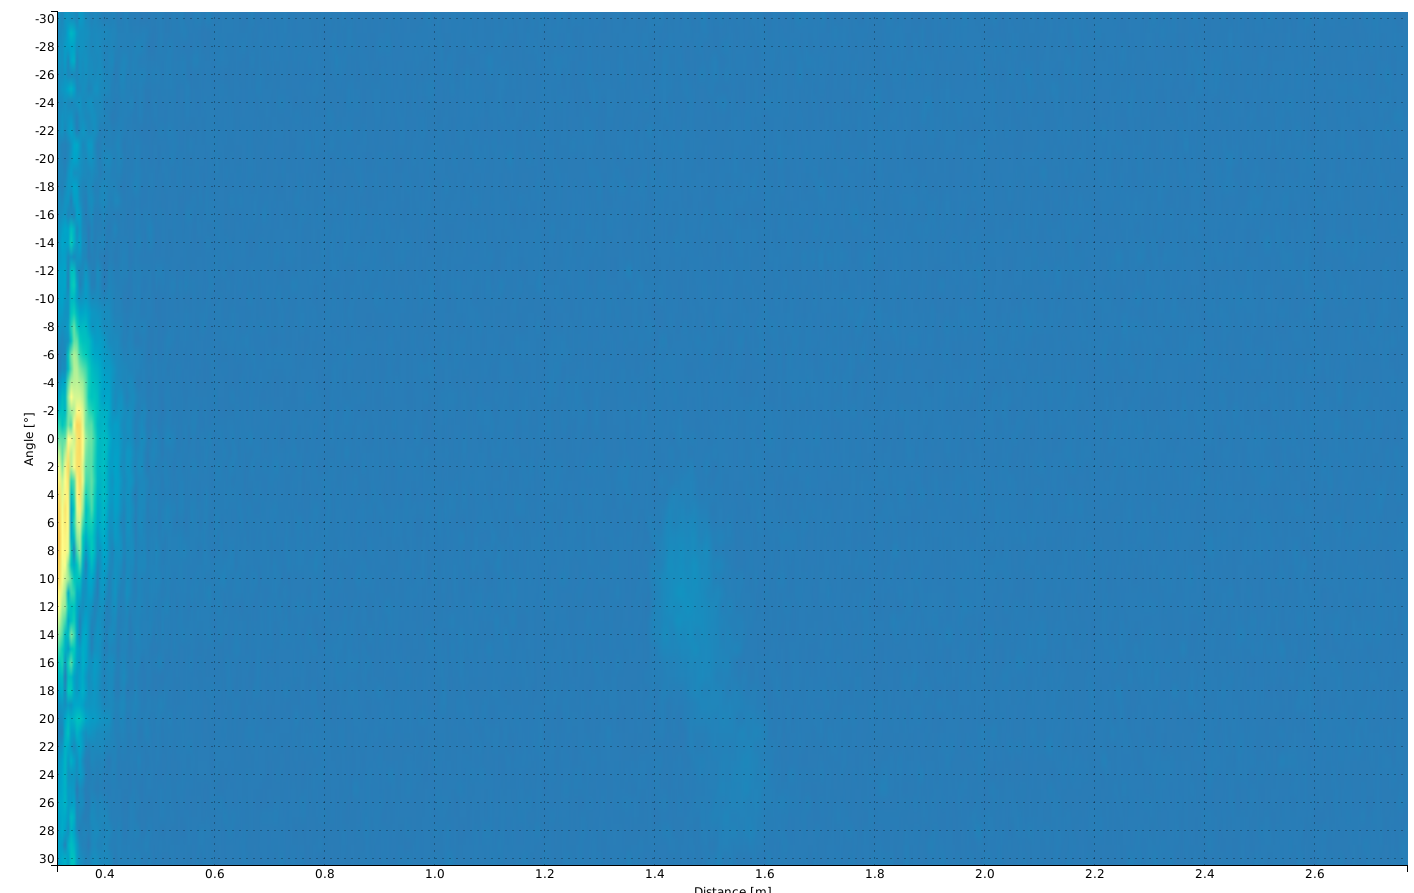
\includegraphics[width=\textwidth]{graphics/image_test_obj_schaumstoff_20deg_1.png}
\caption{Schaumsstoffstück parallel zum Array ausgerichtet} % picture caption
\label{fig:image_test_obj_schaumstoff_20deg_1}
%\end{figure}
%
%(Abb. \ref{fig:image1})
%%%%%%%%%%%%%%%%%%%%%%%%%%%%%%%%%%%%%%%%%%%%%%%%%%%%%%%%%%%%%%%%%%%%%%%%%%%%%%%%
\end{minipage}
\begin{minipage}{1.0\textwidth}
%%%%%%%%%%%%%%%%%%%%%%%%%%%%%%%%%%%%%%%%%%%%%%%%%%%%%%%%%%%%%%%%%%%%%%%%%%%%%%%%
% pictures
%\begin{figure}[htb]
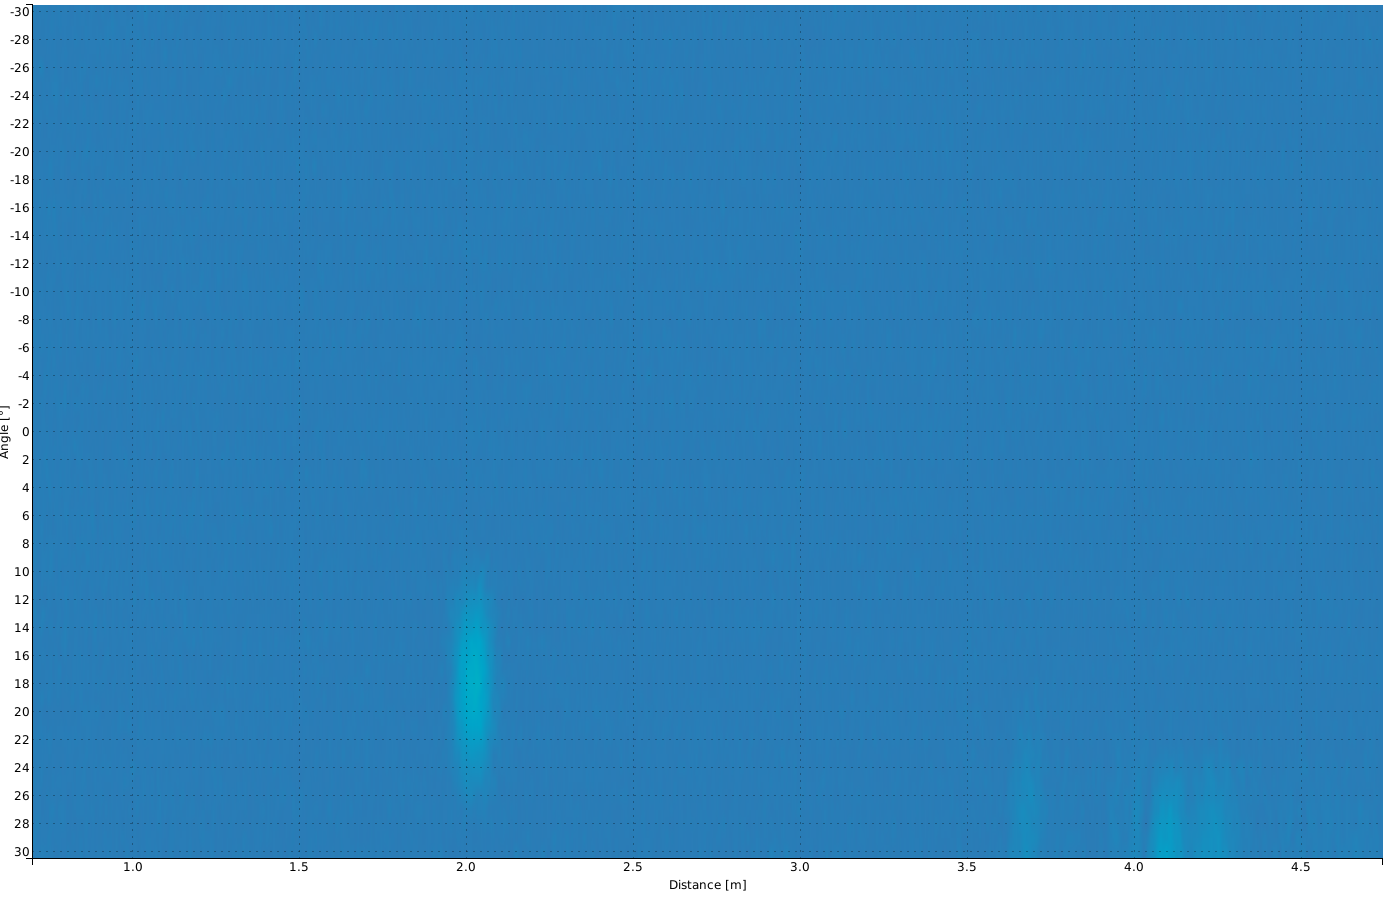
\includegraphics[width=\textwidth]{graphics/image_test_obj_mikrophonstaender.png}
\caption{Mikrophonständer im reflexionsarmen Halbraum mit offener Türe} % picture caption
\label{fig:image_test_obj_mikrophonstaender}
%\end{figure}
%
%(Abb. \ref{fig:image1})
%%%%%%%%%%%%%%%%%%%%%%%%%%%%%%%%%%%%%%%%%%%%%%%%%%%%%%%%%%%%%%%%%%%%%%%%%%%%%%%%
\end{minipage}
\end{figure}
